%!TEX root = ../physical-olympics-2.tex
\setcounter{chapter}{2}
\chapter{稳恒电流}


\section{稳恒电流描述与形成}
\subsection{德鲁特模型}
电荷的定向移动形成\emph{电流}(current).\,就好像一缸气体在慢慢挪动那样,\,电荷的定向移动并不是纯粹的匀速运动,\,而是与无规则的热运动相叠加.\,1900年前后德鲁特({\it P. Drude})和洛伦兹({\it H. A. Lorentz})等人提出\emph{德鲁特模型}(Drude model)来解释金属中的导电现象.\,主要观点是金属内部自由运动的电子类似于理想气体那样做自由的运动,\,称为\emph{自由电子气}(free electron gas).\,我们用电子电量$-e$,\,质量$m$,\,电子数密度$n$,\,和\emph{弛豫时间}(relaxation time)$\tau$,\,平均速度$v$来表示其特征.\,弛豫时间就是电子做匀速直线运动,\,与原子实两次碰撞之间的平均间隔时间.\,与之相关的另一个量还可以是\emph{平均自由程}(mean free path)$\lambda$.\,容易想像,\,典型的情形是,\,常温下电子的平均速度是和气体分子的平均热运动速度那样,\,一个非常巨大的速度,\,而金属原子之间的距离又是那么地短,\,导致电子发生十分频繁的碰撞.\,而如果在金属中加一个电场$\bs{E}$,\,它在两次碰撞内是只可以让电子速度改变一个十分微小的量的:
\[\bs{a}=-\frac{e\bs{E}}{m}\]
\[\bs{v}(0)\quad\longrightarrow\quad\bs{v}(t)=\bs{v}(0)+\bs{a}t\quad\longrightarrow\quad\bs{v}(\tau)=\bs{v}(0)+\bs{a}\tau\]

我们根据统计力学的思想,\,计算在某一时刻电子速度对所有电子取热平衡分布的平均:
\[\bs{u}=\langle\bs{v}\rangle=\langle\bs{v}(0) +\bs{a}t\rangle = \bs{a}\tau\]

上式$t$代表距离上次碰撞每个电子幸存的时间.\,$\bs{v}(0)$代表上次碰撞后其速度.\,一方面,\,认为碰撞使得电子速度完全随机分布,\,平均的结果为零.\,另一方面,\,认为电子的碰撞是一个泊松过程,\,其碰后幸存时间的概率分布是一个指数分布:
\[p(t)=\ue^{-\frac{t}{\tau}}\]

从而平均的$t$为
\[\langle t\rangle=-\int_0^\infty t\ud p=\left. pt\right|^0_\infty+\int_0^\infty \ue^{-\frac{t}{\tau}} \ud t=\tau\]

最后结合电流密度为:
\[\bs{j}=-ne\bs{v}\]

我们得到:
\[\bs{j}=\frac{ne^2 \tau}{m}\bs{E}\]

的结果.\,称为\emph{微观欧姆定律}(microscopic Ohm's law),\,其中系数被称为\emph{电导率}(electrical conductivity):
\[\sigma=\frac{ne^2 \tau}{m}\quad;\quad \bs{j}=\sigma\bs{E}\]

十分值得指出的是,\,作为德鲁特模型的另一个重要结论,\,金属的\emph{热导率}(thermal conductivity)在理论中也可以给出一个估计值.\,我们都知道金属比绝大多数其他固体都拥有好得多的导热性能.\,这可以用热导率与\emph{傅里叶热传导定律}(Fourier's law of thermal conduction)来描述:
\[\bs{q}=-\kappa \nabla T\]

其中$\bs{q}$为热流密度,\,$\kappa$即为材料的热导率.\,水常温下热导率只有$0.591 \rm W/(m\cdot K)$,\,但纯的铜却能够达到$401 \rm W/(m\cdot K)$.\,金属的高热导率全都得益于轻盈的电子气,\,它能够迅速地把局部的热运动加剧传导开来.\,类比理想气体的非平衡态统计方法,\,我们给出:
\[\kappa=\frac{1}{3}nv\lambda c\]

式中$c$为每个电子的动能与温度的比.\,利用$\lambda=v\tau$,\,我们把热导率和电导率做比,\,便可以把较难确定的散射弛豫时间消去,\,得到:
\[\frac{\kappa}{\sigma}=\frac{mv^2c}{3e^2}\]

德鲁特模型认为,\,作为类似于理想气体的电子气,\,理应有:
\[c=\frac{3}{2}k\quad ;\quad \frac{1}{2}mv^2=\frac{3}{2}kT \]

从而得到:
\[\frac{\kappa}{\sigma T}=\frac{3}{2}(\frac{k}{e})^2\]

历史上金属热导率和电导率的比值与温度相关的现象很早就被人们发现,\,一般温度升高时电导率会有十分明显的下降,\,也就是金属的电阻会上升.\,小灯泡在未发光时与正常发光时电阻就经常有2倍左右的差距.\,而1853年魏德曼({\it G. Wiedemann})和弗朗茨({\it R. Franz})观察到不同金属虽然导电导热性能差距悬殊,\,室温下两者之比却接近一个常数,\,称为\emph{魏德曼-弗朗茨定律}(Wiedemann-Franz's law).\,而洛伦茨({\it L. Lorenz})\footnote{注意,\,丹麦物理学家路德维希·洛伦茨({\it Ludvig Lorenz})(1829-1891)与荷兰物理学家亨德里克·洛伦兹({\it Hendrik Lorentz})(1853-1928)是两个不同的人.\,有一个方程以它们两人的名字共同命名:\,Lorenz-Lorentz关系.}在1872则把这一经验规律确定到常数与绝对温度成正比的形式.\,最后德鲁特电子论将这个常数以微观常数的形式确定下来,\,等式右边现在约为$1.11\pow{8} \rm W \cdot\Omega /K^2$,\,这与实验结果数量级是一致的,\,但却差了约2倍.\,真实的值被称为\emph{洛伦兹常数}(Lorentz number):
\[\frac{\kappa}{\sigma T}=L=\frac{\pi^2}{3}(\frac{k}{e})^2=2.44\pow{8} \rm W \cdot\Omega /K^2\]

这个理论很成功,\,但最后的结果的不符合让人感到疑惑.\,还有一个令人感到疑惑的问题.\,就是对于电子气的电容.\,既然电子是完全独立于金属原子实的另一个热力学体系.\,按照经典统计物理.\,原子实的摩尔热容与离子晶体等类似,\,大概在$3R$附近\footnote{即\emph{督龙-裴替定律}(Dulong-Petit Law).}.\,而电子按只有平动自由度的理想气体考虑应贡献$1.5R$热容.\,实验却否定了这一点,\,金属常温下热容仍然是在$3R$附近.\,电子仿佛没有被热激发,\,然而电子又势必参与导热,\,因为金属的导热性能明显优于其他物质.\,那么以上推导过程中哪儿存在不合理之处?\,几年后到来的量子力学革命让人们认识到这一个经典模型从一开始就做了不止一个的与微观实际情况不符的假定,\,但又是十分巧合地,\,最终结果与真实值数量级自动一样了.

\subsection{费米气观点*}

元素周期律引发了人们对原子核外电子排布规律的研究,\,人们惊奇地发现电子是\emph{费米子}(fermion),\,符合\emph{泡利不相容原理}(Pauli exclusion principle).\,这赋予电子独特的量子特性.\,具体来说,\,单位体积内如果电子数目越多,\,那么其最低平均能量就必须越大.\,因为能量最低的状态一旦被占据,\,其他电子就必须占据能量更高的状态,\,即使按照最低能量的方式去堆积(绝对零度时的行为),\,电子也将具有很高的平均能量.\,它符合类似位置-动量不确定性原理的反比率,\,电子浓度的减小了单电子占据的位置尺度,\,则它的动量就会增加,\,从而根据色散关系$p^2=2mE$其能量也会升高.\,这一点使得我们去修改经典的德鲁特模型.\,相应的量子气体称为\emph{费米气}(Fermi gas).

定量计算费米气的特性需要考虑电子的波动本性.\,我们暂时取金属为长宽高为$ABC$的长方体,\,那么如果将$N$个电子倒入这个容器,\,电子的数密度为:
\[n=\frac{N}{ABC}\]

让我们考虑一下电子对状态的填充,\,长方体相当于一个谐振腔,\,事实上给出了电子动量状态的量子化:
\[p_x A=ah\;,\; p_y B=bh\;,\; p_z C=ch\]
\[a,b,c\in\mathbb{N}\]

这是因为根据德布罗意关系$p=\hbar k$而电子状态需要满足$kL=2m\pi$的缘故.\,从而我们发现电子的三个方向的动量都是量子化的.\,量子化的单位为:
\[\Delta p_x=\frac{h}{A}\;,\;\Delta p_y=\frac{h}{B}\;,\;\Delta p_z=\frac{h}{C}\]

\begin{wrapfigure}[16]{o}[-10pt]{7cm}
\centering
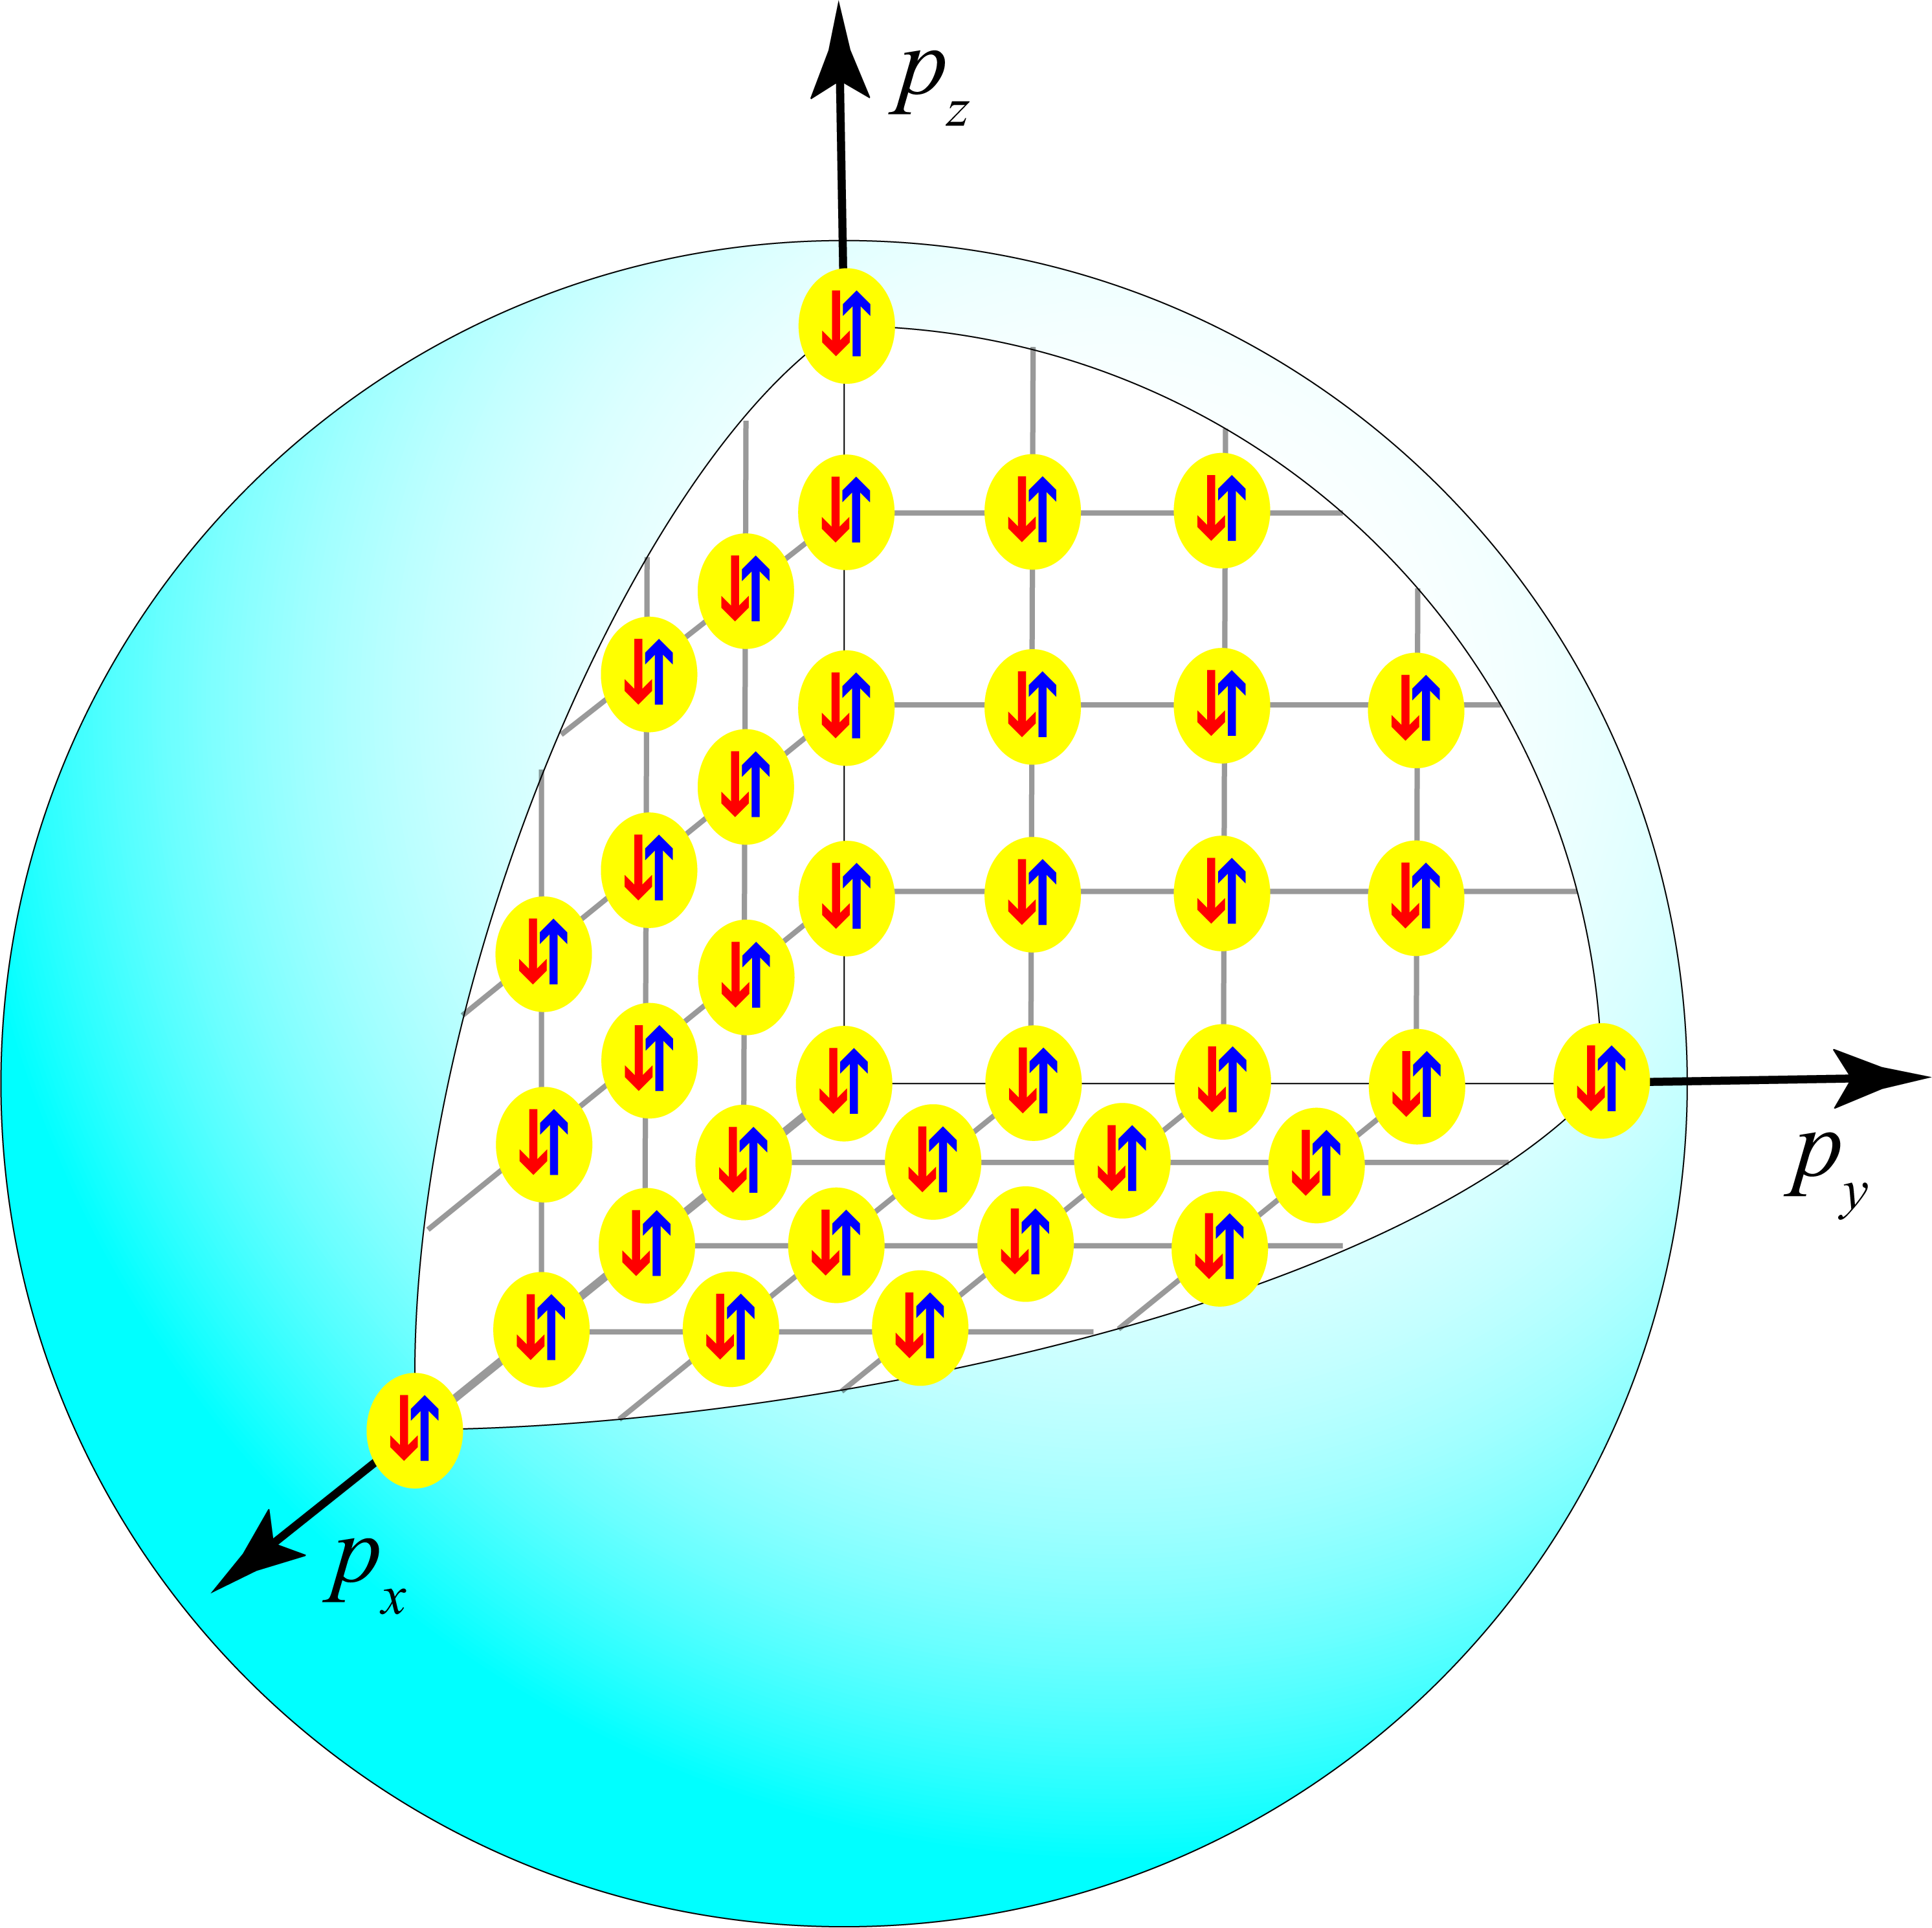
\includegraphics[width=7cm]{image/7-3-1.png}
\caption{电子态密度}
\end{wrapfigure}
现在把$N$个电子倒入动量空间中,\,那么电子在低温下将从最低能量态开始填充,\,由于电子数目巨大,\,最后电子将填充到能量为$\varepsilon_F$处.\,这样的一个填满电子的动量空间中的球体称为\emph{费米海}(fermi sea),\,最终填充到的能量称为费米能级$\varepsilon_F$,\,对应的电子动量为费米动量$p_F$.\,注意到一个动量空间中的一个标志状态的坐标内部实际上有两个独立的态,\,它们表示即使这两个波的波矢$\bs{k}$一样,\,它们代表电子的自旋也不一样\footnote{电子的微观描述是旋量波,\,也就是二分量波函数,\,具有两种可能的自旋.}.\,从而我们写出:
\[2\cdot\left.\frac{4\pi p_F^3}{3}\right/(\Delta p_x \Delta p_y \Delta p_z)=N\]

从而得到:
\[p_F=(\frac{3Nh^3}{8\pi N})^{\frac{1}{3}}=(\frac{3nh^3}{8\pi})^{\frac{1}{3}}\]

在以上过程中总电子数和总体积被消去了,\,最后电子堆积到的动量值仅仅取决于各处电子的数密度而成为了强度量.\,这样一个由于泡利不相容原理所造成的动量值对应到速度上,\,对一般金属估计约为$10^6\rm m/s$.\,而如果按非费米气计算,\,热运动速度应为$\sqrt{kT/m}\sim 7\pow{4}\rm m/s$,\,我们发现经典结果是严重估计少了的.\,但电子的热容又估计多了.\,量子统计给出:
\[c=\frac{\pi^2}{2}k\cdot\frac{kT}{\varepsilon_F}\]

代入热导率公式,\,得:
\[\frac{\kappa}{\sigma}=\frac{\pi^2}{6}\cdot\frac{mv_F^2}{\varepsilon_F}\cdot(\frac{k}{e})^2\cdot T\]

恰好,\,$\varepsilon_F=\dfrac{1}{2}mv_F^2$,\,从而我们得到了正确形式的魏德曼-弗朗茨定律:
\[\frac{\kappa}{\sigma T}=\frac{\pi^2}{3}(\frac{k}{e})^2\]

我们最后做一个经典德鲁特模型与量子费米气模型的比较.\,两个理论都承认以下基本公式的成立:
\[\sigma=\frac{ne^2 \tau}{m}\quad ,\quad \kappa=\frac{1}{3}nv^2\tau c\]

先看电导率,\,经典理论与量子理论对各个参数的估计除了$\tau$其他都是一致的.\,而经典更倾向于对$\tau$的估计更小.\,因为经典理论一般认为$\tau=\lambda/v$,\,而$\lambda$一般就按照原子实之间的平均距离来估计.\,这一点之后就知道是不妥当的,\,因为电子实际上可以在严格周期性的势能场中毫无散射的传播下去.\,而使得电子能够被散射的其实是晶格的缺陷,\,热振动等因素,\,从而一般温度升高,\,$\tau$减小,\,金属的导电性能就大大减弱.\,这给出了金属电阻随温度升高而升高的结论.\,这里经典理论对$\lambda$的过低估计恰好被对$v$的过低估计所抵消掉一部分,\,从而最后$\tau$的值在常温下差距也不大.\,而对于热导率,\,经典理论对$v$的过低估计又恰好被对$c$的过高估计修正,\,精确到了仅仅相差一个常数,\,除了经典理论说不清楚的$\tau$,\,经典与量子的在数量级上是基本符合的.

值得一提,\,热导率描述导热,\,电导率描述导电,\,而导电现象的附效应便是热产生.\,也就是\emph{焦耳热}(Joule heating).\,微观的功率密度
\[\bs{j}=\sigma \bs{E}\quad ,\quad w=\bs{j}\cdot\bs{E}\]

也即:
\[w=\sigma \bs{E}^2=\rho \bs{j}^2\]

其中\emph{电阻率}(resistivity)$\rho$为电导率的倒数.\,上为\emph{微观焦耳-楞次定律}(microscopic Joule-Lenz law).

\subsection{能带论*}

费米气模型在量子力学迅猛发展的几十年后回头看又是过于na\"\i ve了.\,人们发现电子终究是在晶格间传播的波动,\,如果原子实与背景的电子给出了严格的周期性的势能,\,那么如果电子的总机械能小于最大势能,\,那么就成为了束缚态,\,限制在一个原子附近运动而成为原子实的一部分.\,而如果电子守恒机械能大于最大势能,\,就成为不受任何阻碍的传导态.\,动能虽在运动中有所波动,\,但绝不会越来越小.\,描述电子的波函数称为\emph{布洛赫波函数}(Bloch wave function).\,而电子如何去填充怎样的能级?\,\emph{布洛赫}({\it F. Bloch})研究并发现了\emph{能带论}(energy band theory)来替代旧的费米气理论,\,这个理论可以统一地描述导体与绝缘体.

能带论可以看成是电子在单原子外的束缚态特征与传导的自由电子气的特征的一种综合,\,一方面电子在这样的一个周期性势场中的运动其守恒的机械能并不是可以取所有值,\,而是分为可以连续取值的区间:\,\emph{能带}(band)与根本取不到的能量区间:\,\emph{带隙}(gap)所构成.\,而电子作为波动用其所在的能带与波矢$\bs{k}$来描述.\,其波矢方向的物理意义不再重要,\,因为每一个态一般都代表某种驻波与行波的混合,\,而每一个态附近的群速度则可以代表这个态代表的真实电子运动速度.\,另一方面这些能带的结构又恰好对应到了单原子的束缚态能级.\,这使得我们经常是一望某元素的单原子核外电子排布,\,便能从其是否具有最外层电子读出这种元素单质是否能导电的信息.
\begin{figure}[H]
\centering
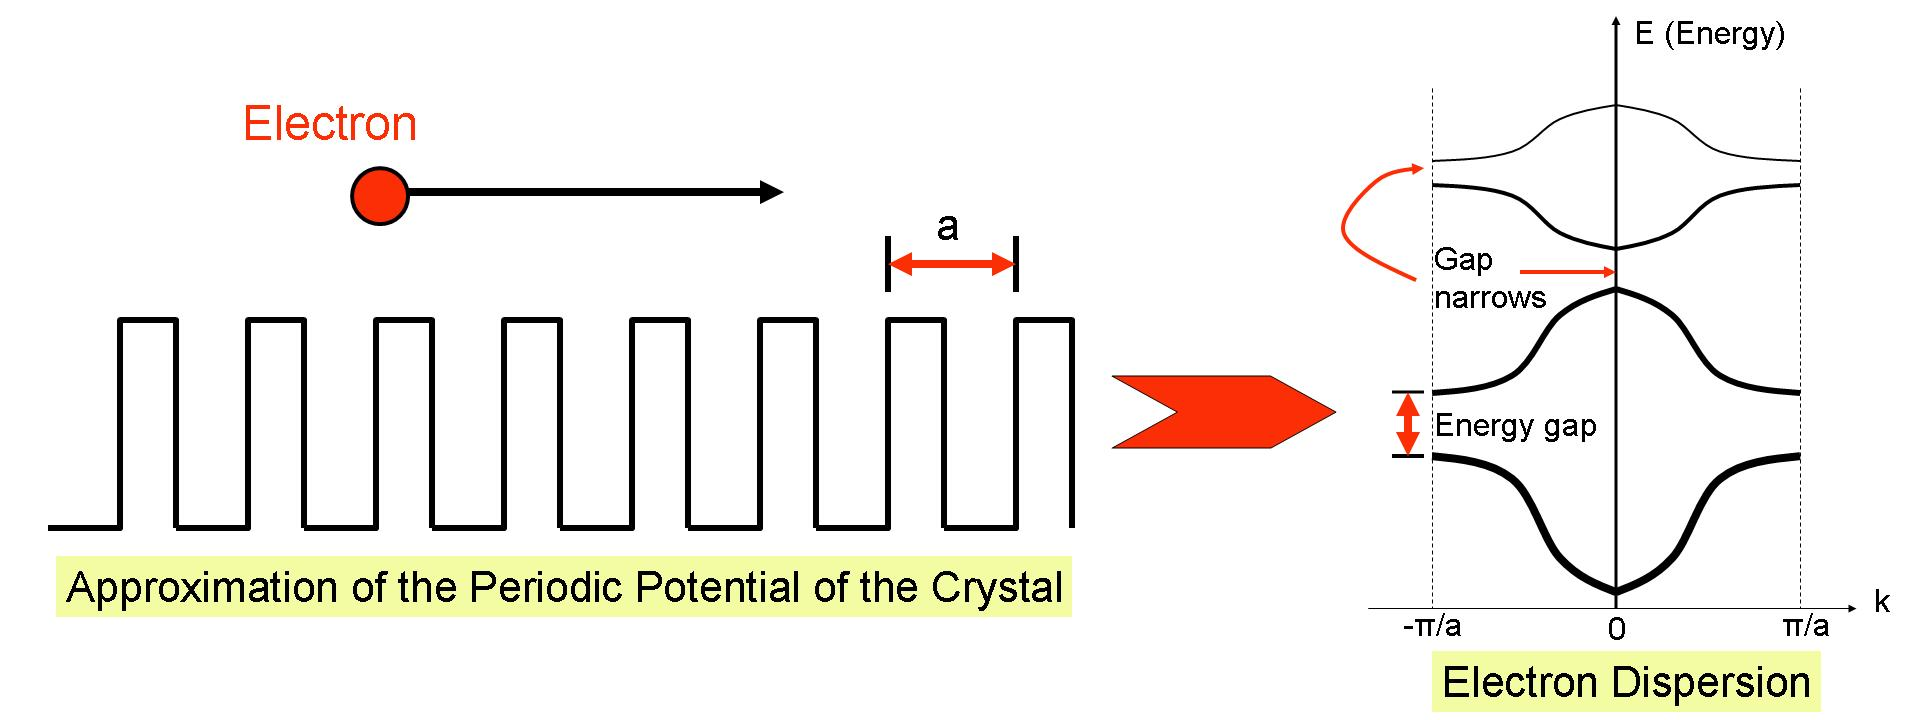
\includegraphics[width=0.8\textwidth]{image/7-3-2.jpg}
\caption{电子在周期性势场中传播}
\end{figure}

某种原子形成晶体时,\,电子从最低的能带开始填充,\,内层电子填满了较低的那些能带,\,它们不参与导电,\,对应于原子实电子和在晶体共价键键合的价电子.\,最外层电子较少的原子,\,形成晶体时最后填充的那个能带没有填满,\,或者虽然填满但与下一个能带在能量区间上重合而能够导电.\,称为\emph{导体}(conductor).\,对应的元素也就显示出明显的金属性\footnote{思考:\,氢是否具有金属性?\,参考\url{https://en.wikipedia.org/wiki/Metallic_hydrogen}.}.\,而若原子外层电子数目多,\,则很有可能电子恰好填满一个能带后隔着一个能隙与空的上方能带相望,\,则所有态都稳定不变,\,材料所有电子都是束缚电子,\,最后填充的那个满带称为\emph{价带}(valence band),\,代表原子间成共价键的价电子所在的能带.\,而上方的那个空带称为\emph{导带}(conduction gap).\,意为一旦这个带中存在电子则会大大改善其导电性能.\,此时元素体现出非金属性,\,一般形成的都是\emph{绝缘体}(insulator).\,而在金属性元素与非金属元素分界处则存在很多的\emph{类金属}(metalloid),\,它们形成的晶体虽然与绝缘体一样,\,在最低能量时恰好把价带排满,\,而隔着一个带隙与空的导带相望.\,但带隙很小(小于$4{\rm eV}$),\,导致常温的热激发和掺杂,\,抑或是光照激发都将在导带中激发大量载流子而具有可观的导电性能.\,这些材料称为\emph{半导体}(semiconductor).
\begin{figure}[H]
\centering
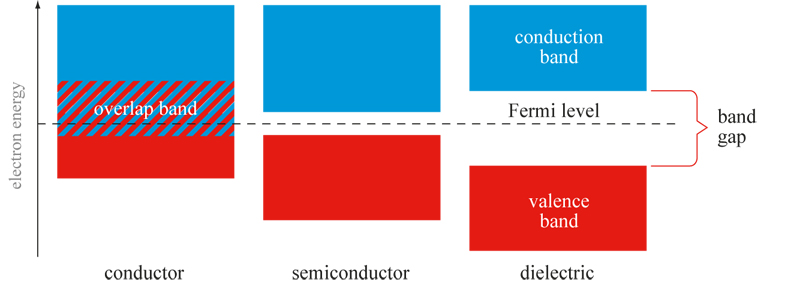
\includegraphics[width=0.8\textwidth]{image/7-3-3.jpg}
\caption{能带与导电性}
\end{figure}
\begin{figure}[H]
\centering
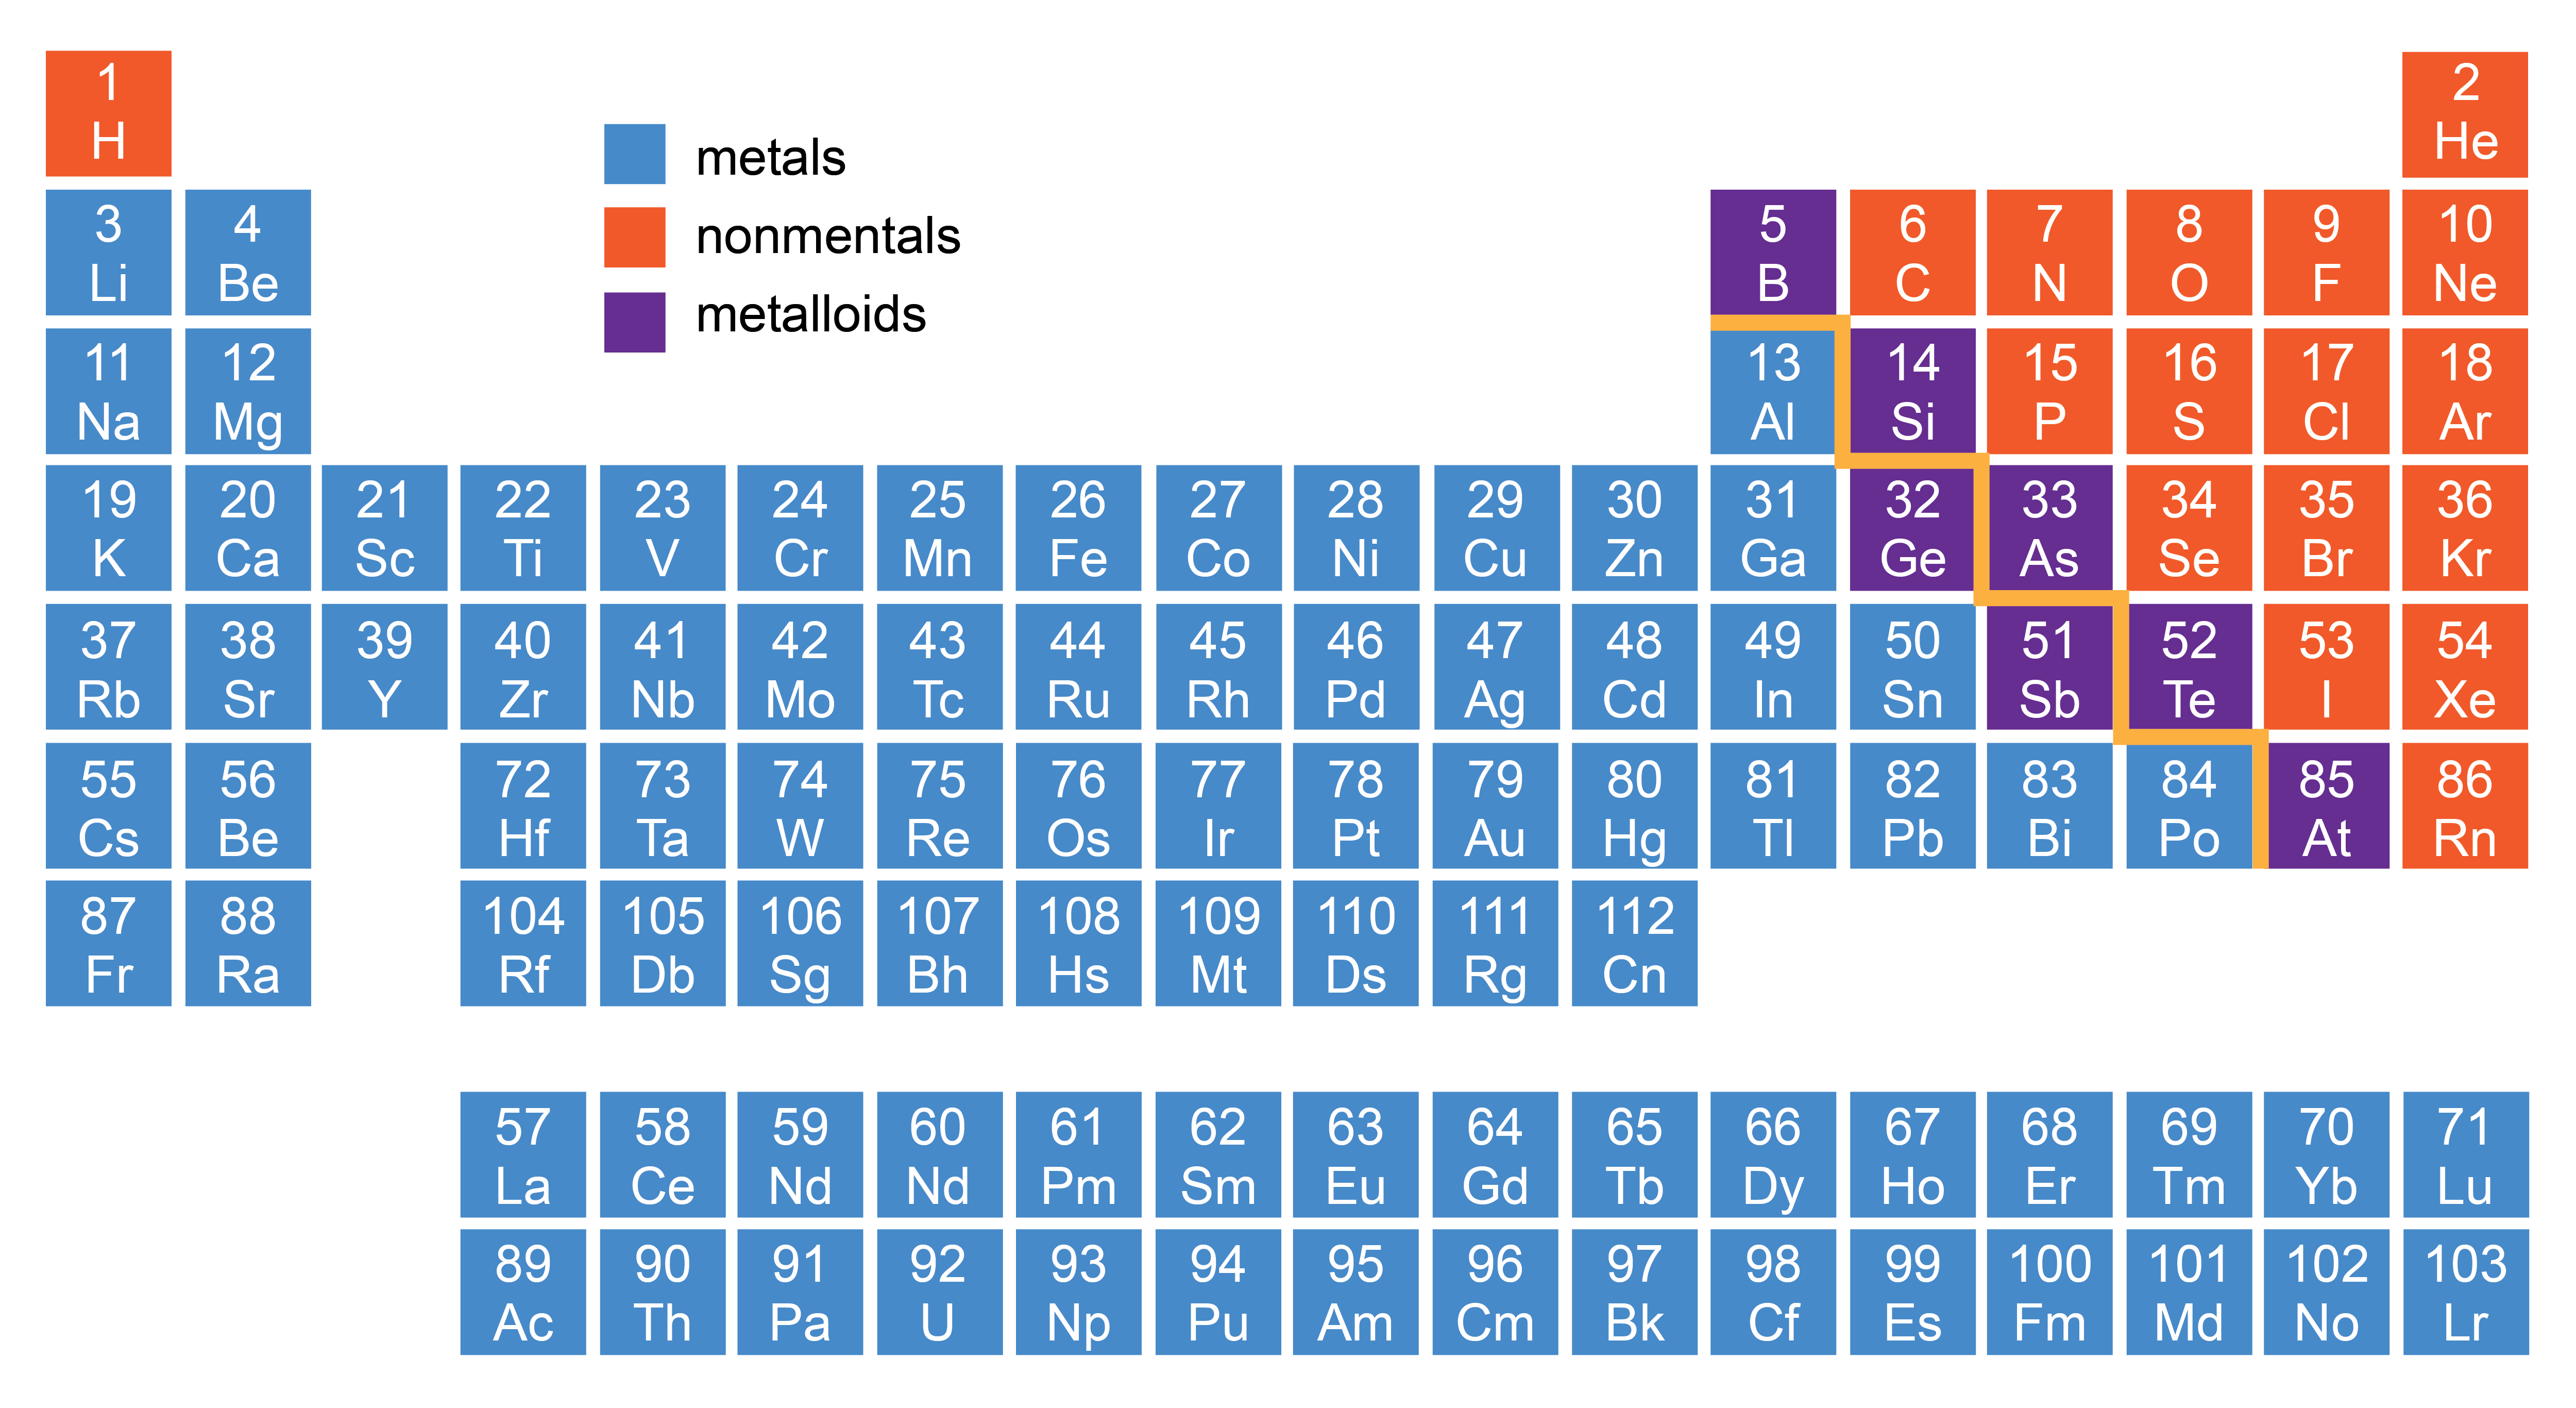
\includegraphics[width=0.8\textwidth]{image/7-3-4.jpg}
\caption{金属,\,类金属与非金属元素}
\end{figure}

那么能带论如何给出电导率的计算公式?\,仍然是:
\[\sigma=\frac{ne^2 \tau}{m}\]

与上一个费米气模型区别在于一点,\,就是这里的$m$不再是电子的\emph{裸质量}(bare mass),\,而是由于与周期性势场相互作用,\,电子的色散关系(能量与波矢关系)被修正后给出的\emph{有效质量}(effective mass).\,即使对于金属,\,这个质量与真实电子质量相差好几倍的现象也是十分普遍的.



\subsection{惯性,\,阻尼与回复力}

在量子力学还未诞生的时期,\,为了解释导体的导电,\,绝缘体的介电现象,\,并适用于任意交变电磁场在介质中的传播,\,色散,\,吸收与散射.\,洛伦兹提出著名的\emph{洛伦兹模型}(Lorentz model)作为德鲁特模型的补充.\,在这儿电子的惯性被重视,\,电子与晶格的碰撞被简化,\,可能的原子实对电荷的束缚被简化为线性回复力.\,也就是洛伦兹用唯象的谐振子类比来解释电子在外场下的行为:
\[m\ddot{\bs{r}}+\gamma \dot{\bs{r}}+ k\bs{r}=-e\bs{E}\ue^{i\omega t}\]

这个模型的解和它对应的各种特性我们将在光学教材里详细讲解.\,在这里我们仅仅讨论导体中的自由电子,\,故$k=0$.\,与导体导电相关的两个因素为:

一是阻尼系数$\gamma$.\,在直流电场下平衡时稳定的电子速度为:
\[\dot{\bs{r}}=-\frac{e}{\gamma}\bs{E}\]

对比更加本质的德鲁特等导电模型的电导公式,\,容易发现这个唯象系数与电导率和基本参量关系为:
\[\gamma=\frac{ne^2}{\sigma}=\frac{m}{\tau}\]

于是我们可以写出在导体上突然加一个不随时间变化的匀强电场后电子的运动的微分方程:
\[m\ddot{\bs{r}}+\frac{m}{\tau} \dot{\bs{r}}=-e\bs{E}\]

它的解为:
\[\dot{\bs{r}}=-\frac{e\bs{E}\tau}{m}(1-\ue^{-\frac{t}{\tau}})\]

我们十分自然地发现定义电子碰撞的弛豫时间恰好与导体对电场响应的弛豫时间相吻合.\,这一点稍微需要一些讨论和修正.\,见下.

第二点我们来讨论表示电子惯性的质量$m$.\,正是它导致了衰减因子$\ue^{-\gamma t/m}$,\,从而造成电路对电场响应的弛豫.\,但如果讨论电路的弛豫,\,或者说电流的惯性,\,有一点是被我们过低地估计了,\,便是自感现象.\,电荷的加速运动形成变化的电流,\,从而与之相伴的是变化的磁场.\,这个变化的磁场反过来给电流一个反向的作用力.\,由于该力正比于加速度,\,故等价于增加了载流子的质量.\,这里的弛豫时间对应直流暂态电路中的$\tau^\prime=L/R$.\,如果一定要理解为电子的惯性质量,\,那么一般比电子的裸质量要大好几个数量级$m^\ast\gg m$.\,从而一般有电路弛豫时间$\tau=m^\ast/\gamma$不等于微观碰撞弛豫时间.

纯粹的导体是否有回复力项?\,显然在以上电子运动方程中不含这一项.\,但注意到如果有回复力项,\,即使外场为零电子也会做振动.\,真实情况会发生这样的现象吗?\,答案是会,\,即\emph{等离子体振荡}(plasma oscillation).\,原因是电子相对于原子实的位移实际上在金属的表面累积了电荷分布,\,从而在内部激发了电场.\,由于频率很高,\,一般要到紫外波段的频率,\,我们可以完全忽略阻尼的影响.\,当电子有位移$\bs{r}$时将形成极化强度\footnote{显然此时``极化强度''描述的非极化电荷,\,而是自由电荷.}:
\[\bs{P}=-ne\bs{r}\]

我们考虑块状金属板\footnote{的确,\,取不同形状的物体这个频率会有所不同.}的集体等离子体振荡,\,那么由于金属表面的累积电荷在金属内部形成的电场为:
\[\bs{E}=\bs{E}_{\rm in}=-\frac{\bs{P}}{\varepsilon_0}=\frac{ne\bs{r}}{\varepsilon_0}\]

代入原方程:
\[m^\ast \ddot{\bs{r}}=-e\bs{E}=-\frac{ne^2\bs{r}}{\varepsilon_0}\]

从而得到谐振子方程.\,振荡频率为:
\[\omega_p=\sqrt{\frac{ne^2}{\varepsilon_0 m^\ast}} \quad;\quad\sigma=\varepsilon_0\omega_p^2\tau\]

最后我们考虑低频电磁波(内部实际场强)下金属的电子行为,\,利用光学中讨论过的洛伦兹模型,\,我们计算金属的复电容率,\,最后得到:
\[\varepsilon_r(\omega)=1-\frac{\omega_p^2\tau^2}{1+\omega^2\tau^2} \quad ; \quad \sigma(\omega)=\frac{\sigma}{1+\omega^2\tau^2}\]

一般$\omega_p\tau\gg 1$,\,故低频下金属的介电常数实际上是绝对值很大的负数.\,电导率随着频率的增加而减小.


\subsection{稳恒电流与形成条件}

作为电荷的流动,\,电流密度与电荷密度间满足电荷守恒定律:
\[\nabla\cdot\bs{j}+\frac{\partial\rho}{\partial t}=0\]

而所谓\emph{稳恒电流}(steady current)指的是一定区域内导电物质形成的电荷,\,电场,\,电流分布.\,其中电流的分布不能随时间变化,\,自然的结论是电荷密度分布也不能随时间变化.\,否则将产生随时间变化的电场,\,电场造成电流的变化.\,即上式必有:
\[\frac{\partial\rho}{\partial t}=0\quad;\quad \nabla\cdot\bs{j}=0\]

即在稳恒电流中电流密度是一定没有散度的,\,无头无尾的闭合曲线.\,稳恒电流必须是\emph{直流}(direct current)而非\emph{交流}(alternating current).

容易发现,\,在稳恒电流中微观欧姆定律写成以下形式是不完整的:
\[\bs{j}=\sigma \bs{E}\]

在很多情况下,\,上式并没有问题.\,$\bs{E}$被理解为由电荷分布$\rho$形成的静电场\footnote{实际上,\,不包括涡旋电场,\,因为它被归于之后引入的非静电力.\,换句话说,\,这里的$\bs{E}$不再由静止电荷的受力$\bs{F}/q$去定义,\,而是单纯根据静止电荷分布产生平方反比的电场叠加去定义.},\,它是一定可以引入电势的:
\[\bs{E}=-\nabla\varphi\]

\begin{wrapfigure}[13]{o}[-10pt]{8cm}
\centering
\vspace{-0.3cm}
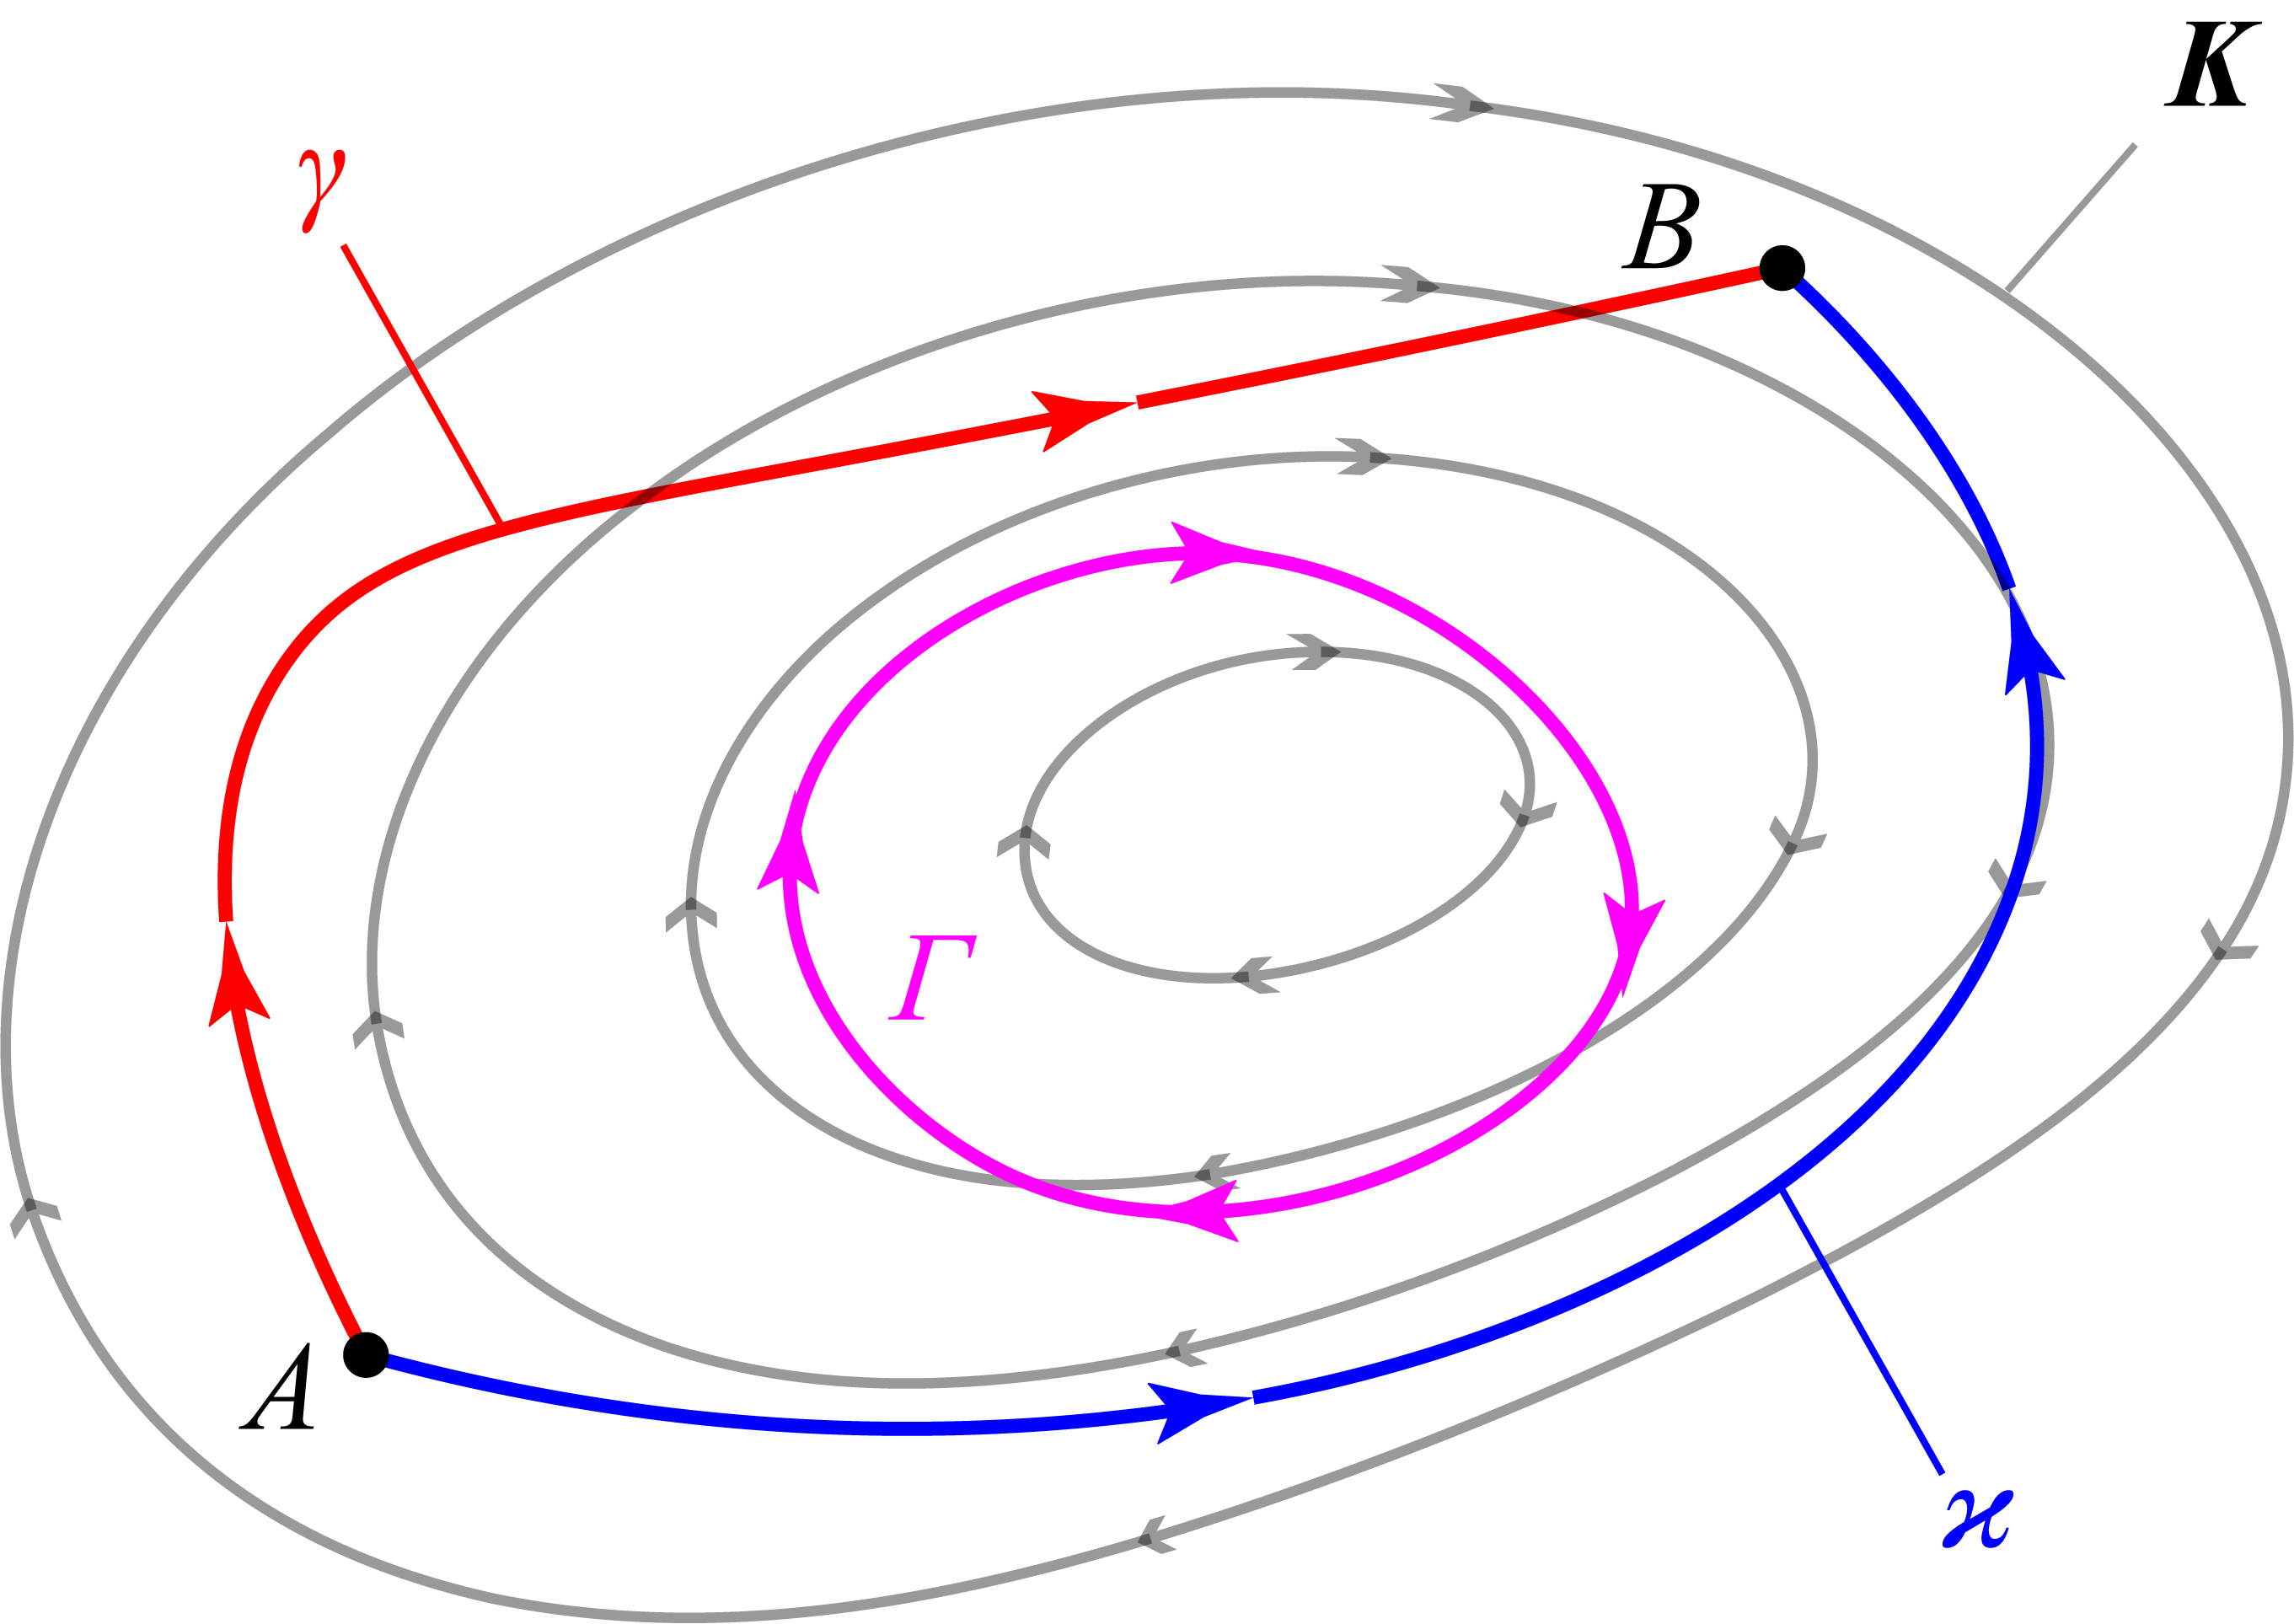
\includegraphics[width=8cm]{image/7-3-5.png}
\caption{非静电场}
\end{wrapfigure}
那么如果承认以上形式的微观欧姆定律就会引起矛盾:\,电流线是环状闭合的,\,电场线必须与电流线同向平行,\,但电场线又不能是闭合的,\,否则与静电场环路定理,\,电势的可定义性矛盾.\,实际上,\,微观形式的欧姆定律必须被写成:
\[\bs{j}=\sigma (\bs{E}+\bs{K})\]


上式$\bs{K}$代表\emph{非静电力场}(non-electrostatic field)对电子产生的作用.\,定义方式与电场量纲一致,\,都是单位正电荷的受力.\,这么写的不同之处就在于,\,把驱动电流的力分成了两部分:\,静电场$\bs{E}$是保守的,\,可以引入势的,\,在一个回路中不做功的,\,不吞吐能量的场(注意电流本身就会发热,\,这不是场造成的而是电荷定向流动碰撞晶格造成的).\,但非静电力就是源源不断做功驱动回路中电流流动的,\,非保守的,\,不能引入势来描述的场.\,虽然不能引入电势来描述非保守力,\,但可以用\emph{电动势}(electromotive force)来描述非静电力:
\[\mathscr{E}_\gamma=\int\limits_{A\stackrel{\gamma}{\longrightarrow}B} \bs{K}\cdot\ud\bs{r}\quad;\quad \mathscr{E}_\varGamma=\oint\limits_{\varGamma}\bs{K}\cdot\ud\bs{r}\]

不像对静电场的积分那样仅仅取决于端点,\,电动势与积分路径一一对应.\,回路电动势一般来说不为零,\,从而相同端点的两个路径电动势也不一定相等:
\[\mathscr{E}_\varGamma\neq 0\quad;\quad \mathscr{E}_\gamma\neq\mathscr{E}_\varkappa\]

非静电力既然能够作用在电子上,\,其形式一般就是电磁力,\,万有引力,\,或是惯性力.\,磁场力对应\emph{动生电动势}(motional emf),\,而由于变化的磁场激发的涡旋电场部分的电场力对应\emph{感生电动势}(transformer emf).\,电子会受到引力,\,1967年Schiff指出电子会因为引力的原因聚集到金属的底部.\,而后Dessler提出了严格的考虑晶格在重力场下压缩与不均匀情况下的电子平衡情况.\,引力是很弱的保守力,\,对金属内部电荷体系的影响虽然很小但绝不是不可观测.\,而与引力类似的惯性力则可以人工制造出很大的数值,\,而且可以使它非保守.\,试想加速旋转一个线圈,\,那么在随晶体加速的参考系里电子受到的角向惯性力就和受到一个电场力造成的效果没有本质的区别.

\begin{wrapfigure}[13]{o}[-10pt]{8cm}
\centering
\vspace{-0.5cm}
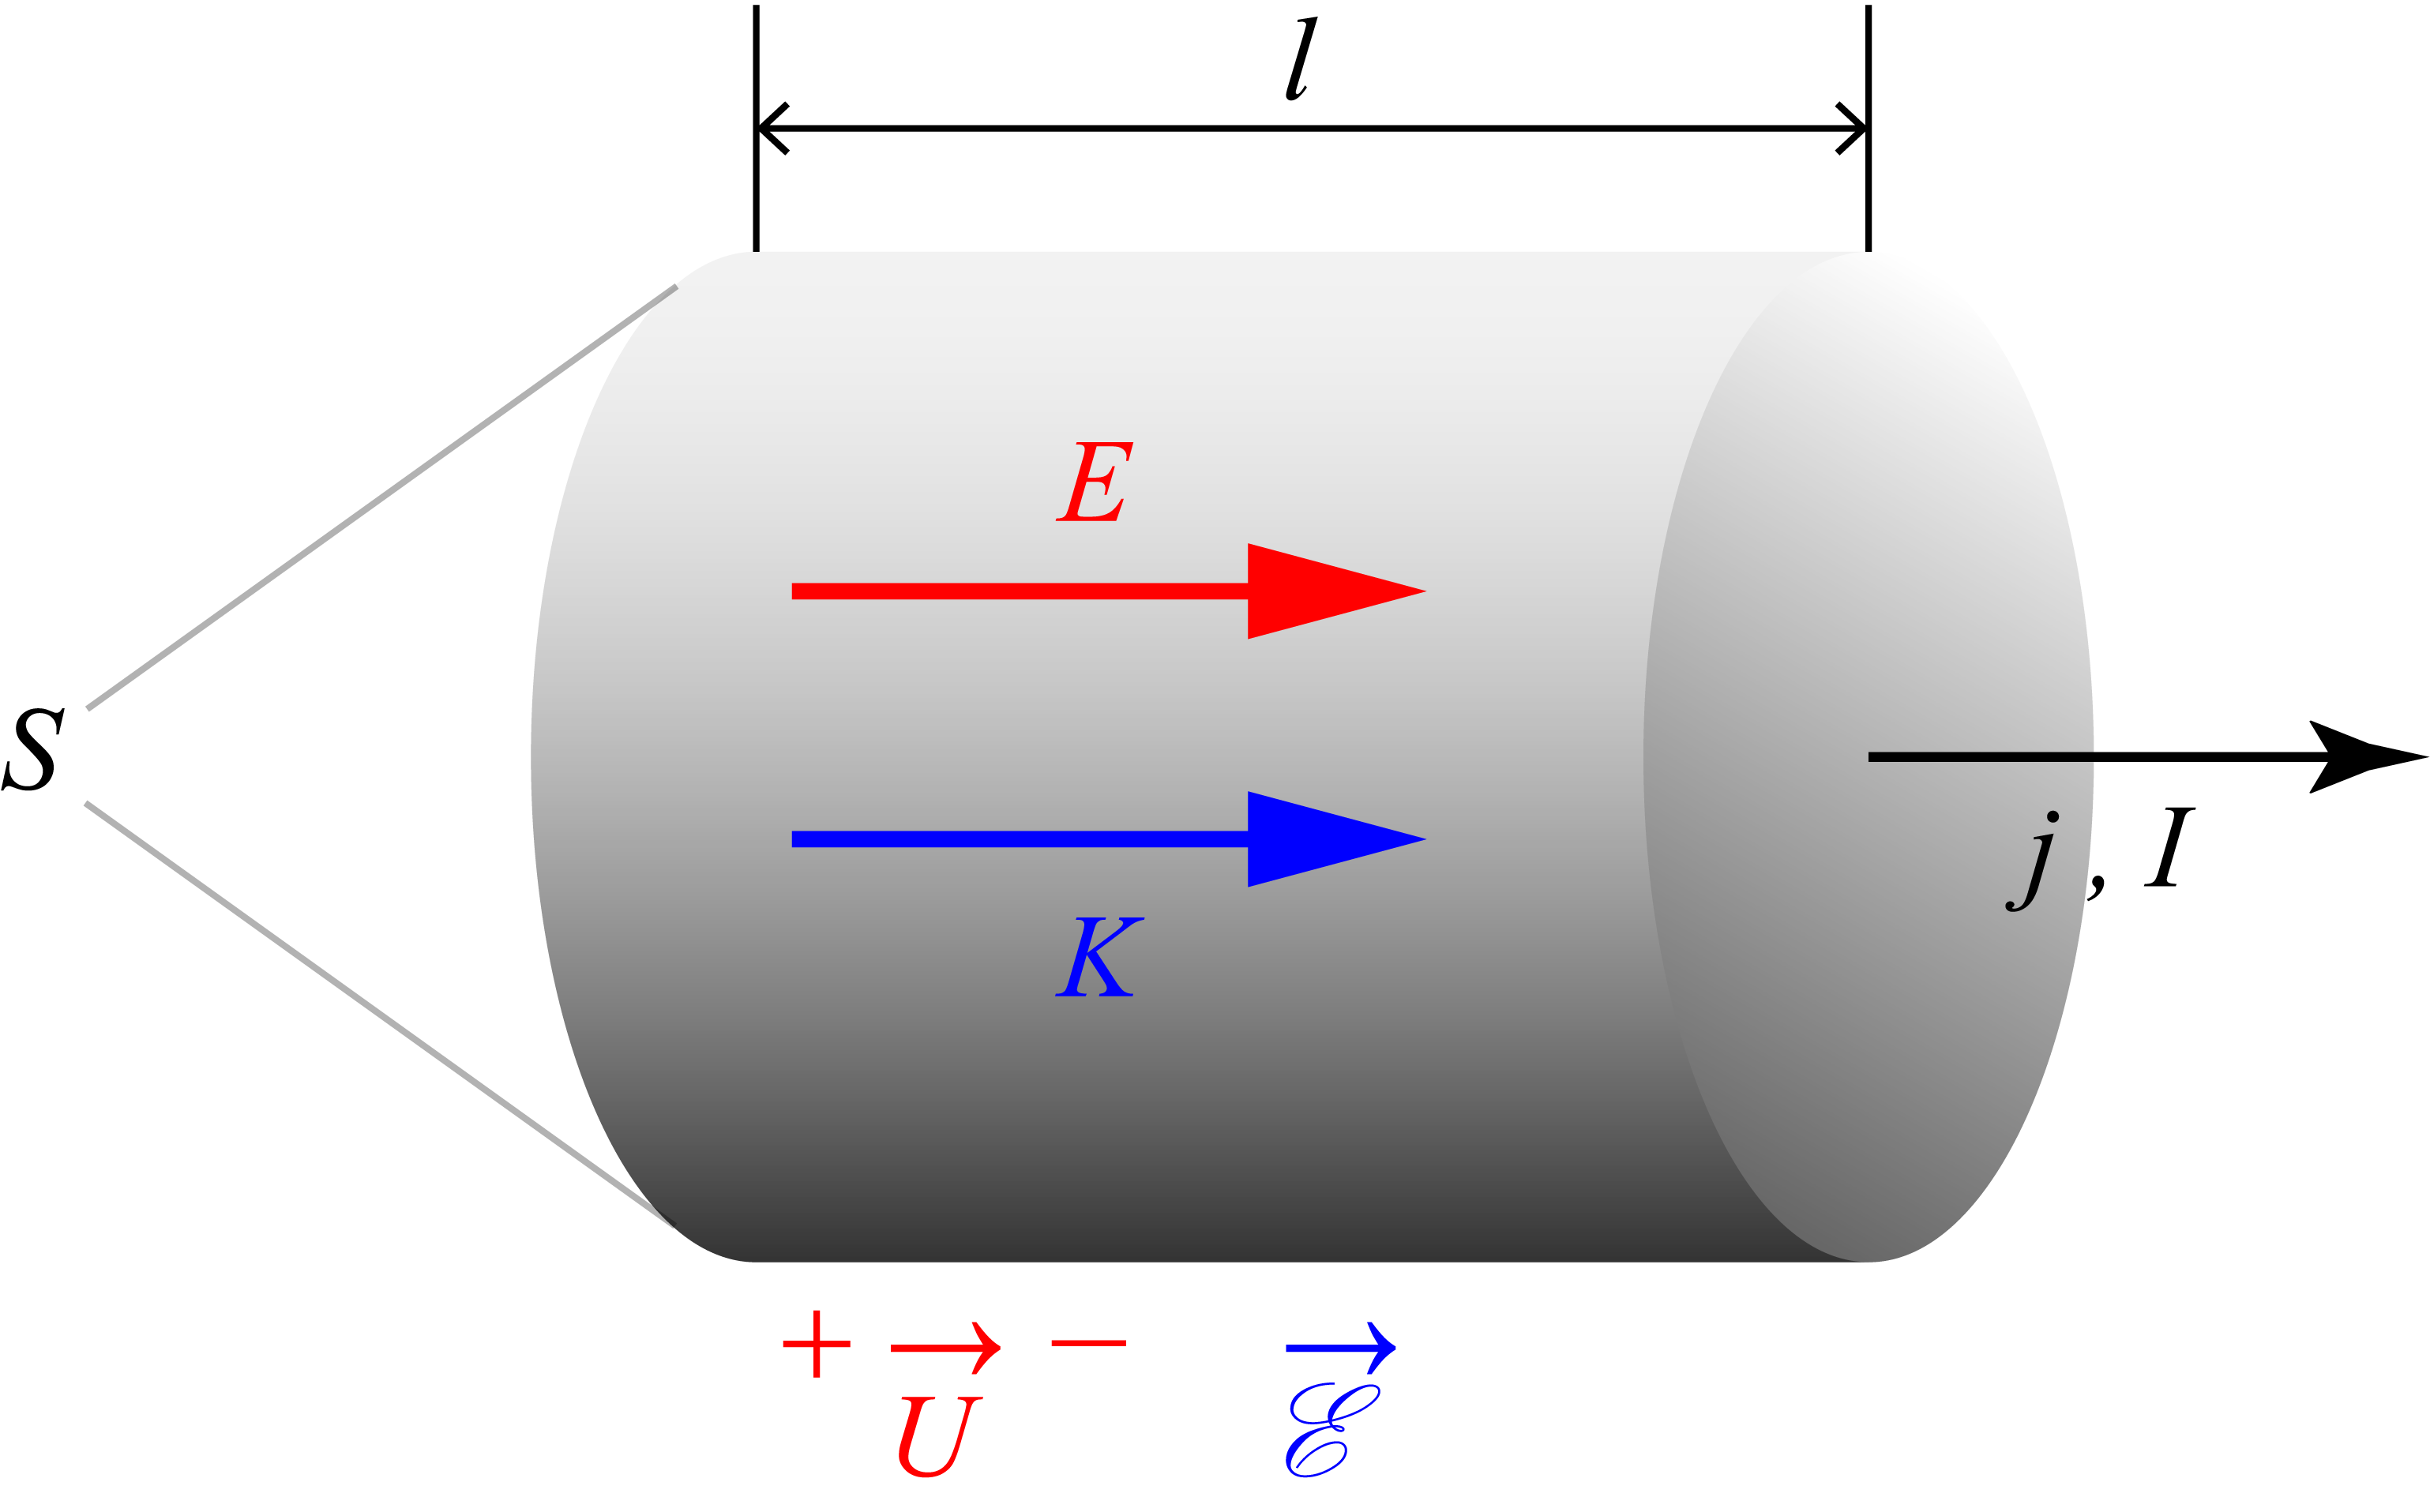
\includegraphics[width=8cm]{image/7-3-6.png}
\caption{宏观欧姆定律}
\end{wrapfigure}
还有一些电动势一般无法用非静电力描述.\,因为在一个回路中某些部分的确有能量的输入,\,但不是以作用在某些具体的电荷上的力的形式.\,而是更加广义的一些力作用在一些流上.\,例如温差电偶利用两种物质的电子的热扩散性质差异,\,从高温端吸取热量而驱动电流.\,化学反应更是源源不断地产生新的物质,\,利用反应的自发性而驱动物质做定向的移动形成电流.\,在这些抽象的场合,\,我们采用某段电路中移动单位电荷,\,外界向体系注入的能量来定义电动势:
\[\mathscr{E}=\frac{\ud W}{\ud Q}\]

\begin{figure}[H]
\centering
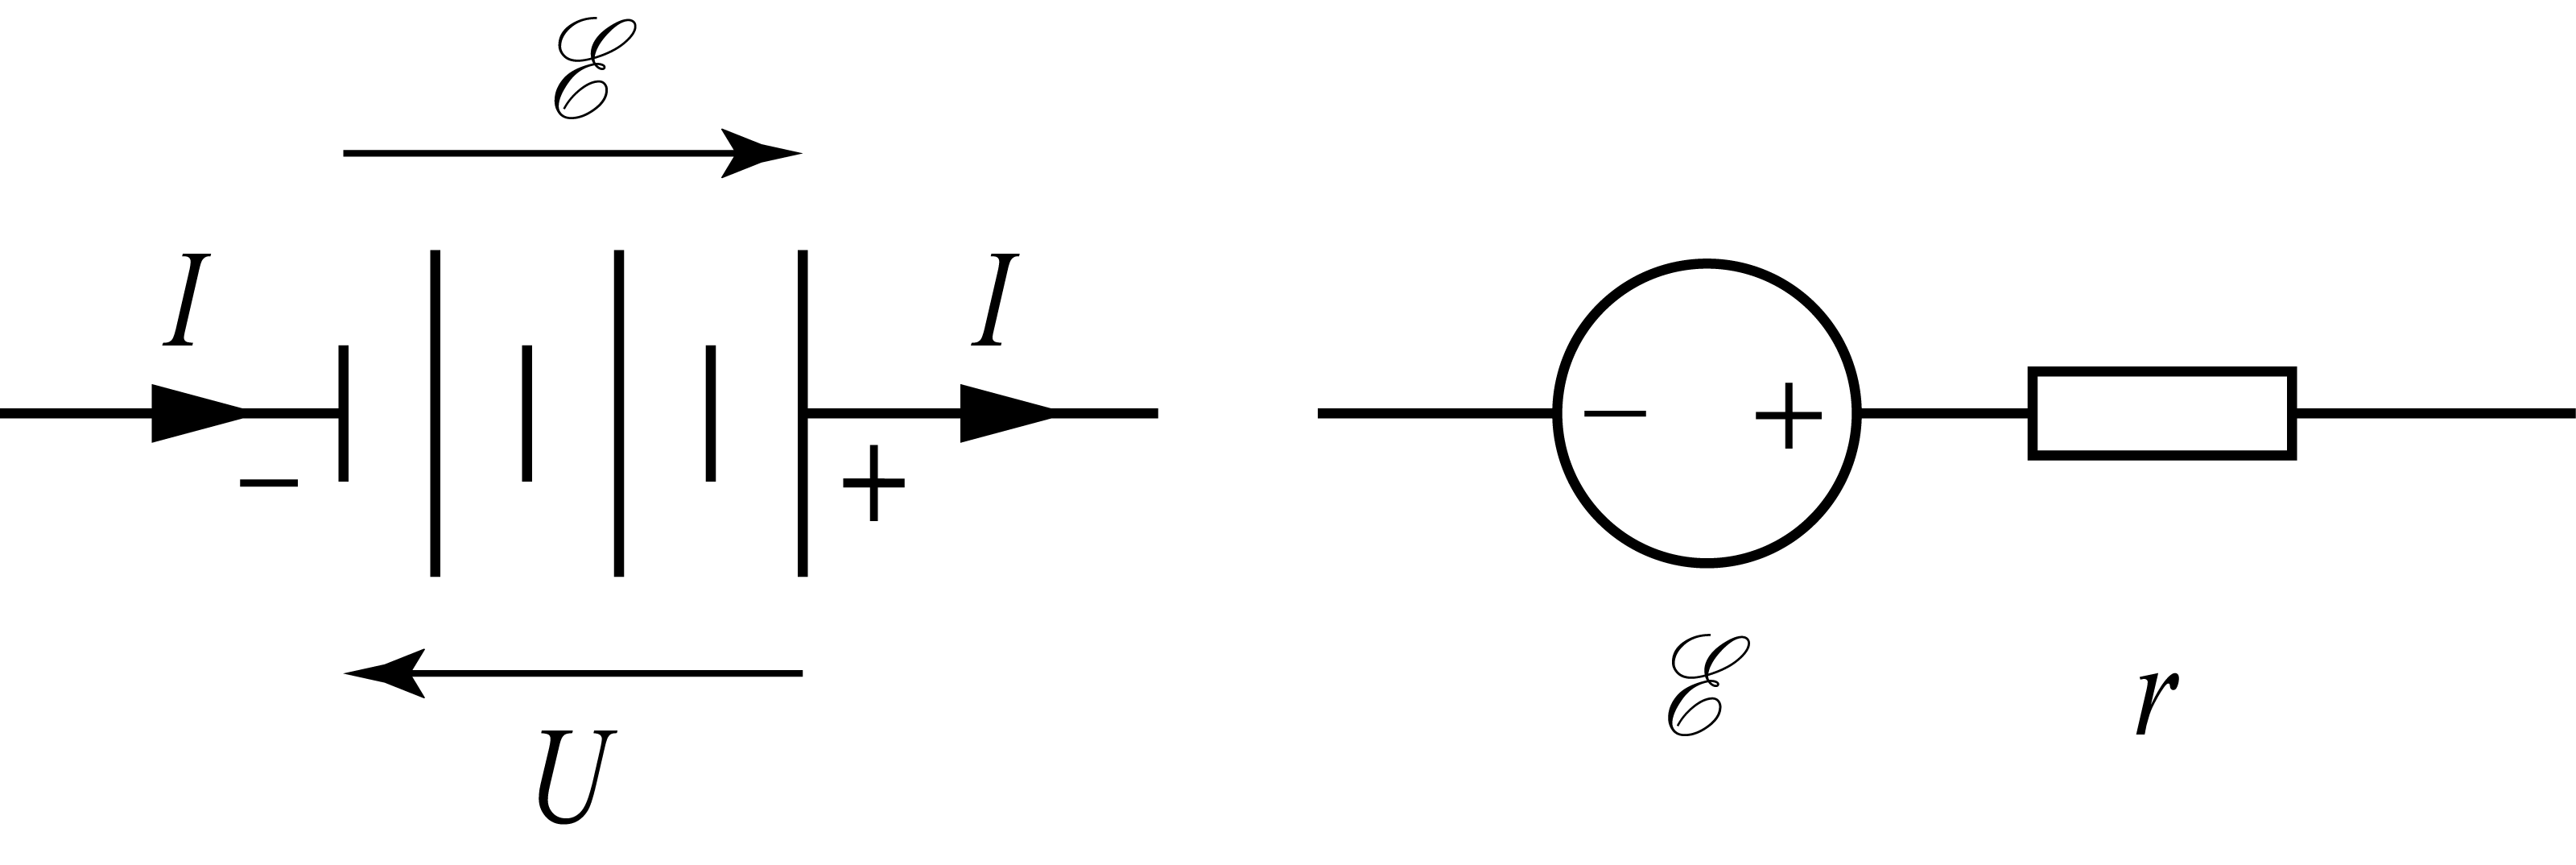
\includegraphics[width=0.6\textwidth]{image/7-3-7.png}
\caption{电池的欧姆定律}
\end{figure}
最后,\,从微观到宏观,\,我们考虑一段长为$l$,\,面积为$S$,\,电阻率为$\rho$的导体上的欧姆定律:
\[E+K=\rho j\]

等式两边同时乘以$l$,\,把电流密度写成$I/S$.\,得到:
\[U+\mathscr{E}=IR \quad;\quad R=\rho\frac{l}{S}\]

一般叫做部分电路的欧姆定律.\,而如果考虑\emph{电池}(battery)的两端,\,正常工作时一般正极电压更高,\,故约定电动势与电压取相反的方向,\,电流则与电动势方向一致,\,却与电压方向反向:
\[U=\mathscr{E}-Ir\]

为一段含源电路的欧姆定律.\,此时我们把电池等效为理想电压源和一个定值电阻$r$的串联.\,电阻即为电池的\emph{内阻}(internal resistance).






\section{电路与电路方程}

具体到直流电路中,\,我们一般提供以下理想的电路元件:
\begin{figure}[H]
\centering
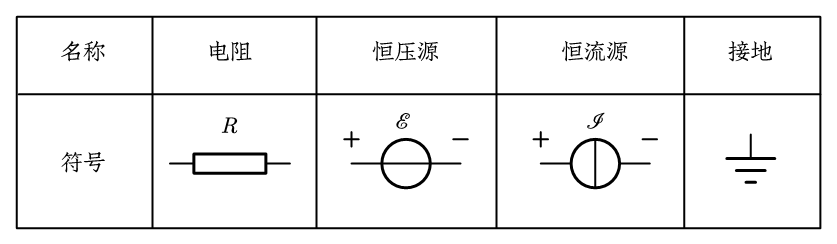
\includegraphics[width=0.7\textwidth]{image/7-3-8.png}
\caption{常见电路元件}
\end{figure}

实际电路总是由这些元件和导线构成,\,导线和元件的内阻均被用实际电阻显式表示.\,接地符号可以被视作特殊的导线.\,一般与真实的``地面''没有任何联系,\,电路中一般``地''指的是公共的零电势参考点.\,电路中如果仅仅有一个接地符号,\,就把接地的点的电势认为是零.\,如果出现了多个接地符号,\,就用导线把这些点连接到同一个点,\,并把这个点电势视作零.

\begin{wrapfigure}[12]{o}[-10pt]{8cm}
\centering
\vspace{-1cm}
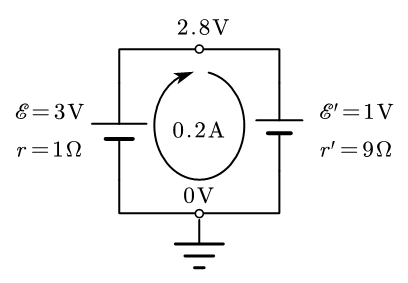
\includegraphics[width=8cm]{image/7-3-9.png}
\caption{相关方向}\label{fig7-3-9}
\end{wrapfigure}
任何一个元件,\,或者二端的部分电路,\,为了研究的统一性与方便,\,我们规定两端的电压的正方向与流过的电流的正方向都取``相关方向'',\,沿着这个方向,\,元件或部分电路表现的像一个电阻,\,或者宽泛一点说,\,像一个用电器.\,即电流就是沿这个方向流动,\,而且电压也沿这个方向降低.\,比如在如图\ref{fig7-3-9}所示的左侧大电池为右侧小电池充电的过程中,\,右侧电路对上下两端口以向下为电压电流的相关参考方向,\,则电压和电流分别为:
\[U=+2.8{\rm V}\quad ,\quad I=+0.2{\rm A}\]

但如果对左侧电路依然取向下为电压电流的相关参考方向,\,则电压和电流分别为:
\[U=+2.8{\rm V}\quad ,\quad I=-0.2{\rm A}\]

可以发现,\,如果一个元件或部分电路按照相关方向计算的电压电流同时是正或者负,\,这个元件就是\emph{类用电器}的,\,整体效果是消耗电能,\,而如果一正一负,\,就是\emph{类电源}的,\,整体效果是产生电能.

在具体分析复杂电路时,\,顺次串联的各个部分电路相关方向一般取为同向;\,讨论单个回路时,\,各个部分的相关方向也是按照某种环绕方向确定的;\,多个二端电路并联在两点之间也通常取各个支路为统一约定的从一个点到另一个点的相关方向.

对于之前的三种元件,\,电阻由于对称性没有天生的电压电流相关方向.\,无论如何取相关方向,\,其电压$U$,\,电流$I$和其参数电阻$R$都一定要满足下式,\,称作\emph{伏安特性}(V-A characteristic):
\[U=IR\]

恒压源,\,顾名思义,\,总是能保持其正极电压比负极电压高$\mathscr{E}$.\,在正常工作状态时,\,电流应当从正极流出,\,使得其成为类电源的元件.\,取此时电流方向为其相关方向(具体问题中相关方向也可以与之相反),\,则其特性为:
\[U=-\mathscr{E}\quad ,\quad I>0\]

理想的恒压源同样能够工作在$I<0$的类用电器区域,\,此时同样有$U=-\mathscr{E}$.\,但是对理想电压源短路是没有意义的,\,一般恒压源所在支路一定需要串联电阻.

恒流源,\,顾名思义,\,总是能保持从负极向正极输出电流$\mathscr{I}$.\,在正常工作状态时,\,正极电压应当比负极电压高,\,使得其成为类电源的元件.\,取此时电流方向为其相关方向(具体问题中相关方向也可以与之相反),\,则其特性为:
\[I=\mathscr{I}\quad ,\quad U<0\]

理想的恒流源同样能够工作在$U>0$的类用电器区域,\,此时同样有$I=\mathscr{I}$.\,但是对理想电压源开路是没有意义的,\,一般恒流源所在支路一定需要并联电阻.


所以我们考虑的电路中,\,如果出现恒压源或恒流源,\,一般以以下带分压内阻或分流内阻的形式存在,\,如果考虑整个元件的特性,\,就给出了著名的\emph{输出特性}(output characteristic):
\begin{figure}[H]
\centering
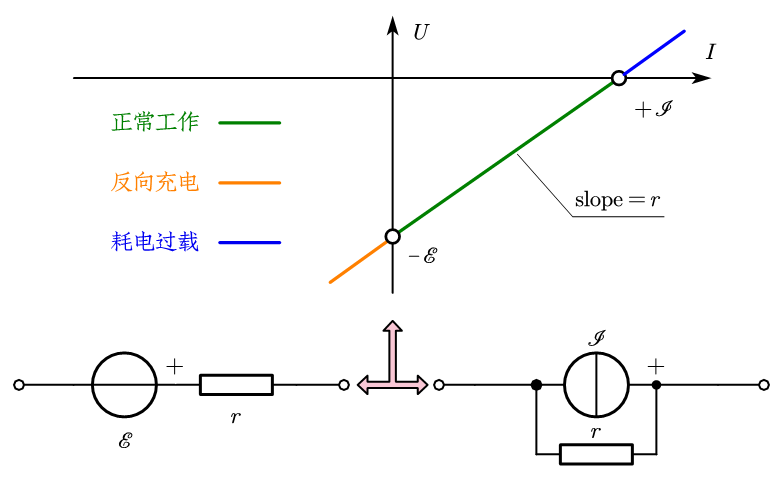
\includegraphics[width=0.5\textwidth]{image/7-3-10.png}
\caption{源的统一输出特性}
\end{figure}
\vspace{-1.5cm}

\[U=-\mathscr{E}+Ir=(I-\mathscr{I})r\]

我们也从中发现了,\,如果恒压源与恒流源满足内阻相等都是$r$且$\mathscr{E}=\mathscr{I}r$,\,那么它们的输出特性是完全一致的.\,也就从功能上等价且可以相互替代,\,这是我们之后小节要介绍的戴维南-诺尔顿定理的一个预兆.\,但这主要只有理论价值,\,实际情况分压内电阻总是要求很小,\,分流内电阻总是要求很大,\,这样在较大输出范围内才能凸显其恒压恒流的特性.

\vspace{1cm}

我们只有三种元件(电阻,\,带内阻的恒压源,\,带内阻的恒流源),\,而且已经成功给出了三种元件的特性,\,它们实际上就是元件上取相关方向以后电压与电流之间的函数关系,\,从而只要知道电流或电压中的一者就可以表示出另一者来.\,但是如果涉及到电路的求解,\,就需要把不同的元件联系起来.\,此时还会涉及到两类方程.\,分别称作\emph{基尔霍夫电流定律}(KCL,\,Kirchhoff's current law)与\emph{基尔霍夫电压定律}(KVL,\,Kirchhoff's voltage law).

\begin{figure}[H]
\centering
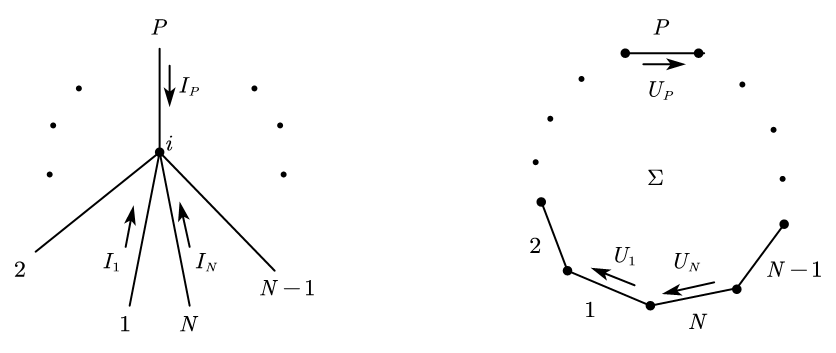
\includegraphics[width=0.6\textwidth]{image/7-3-11.png}
\caption{KCL与KVL}
\end{figure}

KCL的含义是,\,如果多个元件的一端连在一点.\,那么取指向或背离公共节点的方向为所有元件的相关方向,\,必有:
\[\sum_{P\in i} I_P=0\]

我们约定小写拉丁字母$i,\,j,\,k\cdots$用来表示点,\,大写拉丁字母$P,\,Q,\,R\cdots$用来表示元件所在的支路(边),\,而从属符号$\in$用来表示结合关系,\,$P\in i$念做``边$P$以$i$为端点''.\,KCL因此也称作\emph{节点电流定律}.

KVL的含义是,\,如果多个元件的首尾相连构成回路.\,那么取顺时针或逆时针方向为所有元件的相关方向,\,必有:
\[\sum_{P\in \Sigma} U_P=0\]

我们约定大写希腊字母$\Sigma ,\,\Pi,\, \Phi\cdots$用来表示回路,\,同样用从属符号$\in$用来表示结合关系,\,$P\in \Sigma$念做``边$P$在回路$ \Sigma$上''.\,KVL因此也称作\emph{回路电压定律}.

而需要注意的是,\,KCL与KVL都可以以元件电流或电压作为自变量.\,比如用电流做为KVL方程的自变量就构成了所谓的数电压法.\,下图所示的电路回路使用数电压法列顺时针方向的KVL方程就如右式:

\begin{figure}[H]
\centering
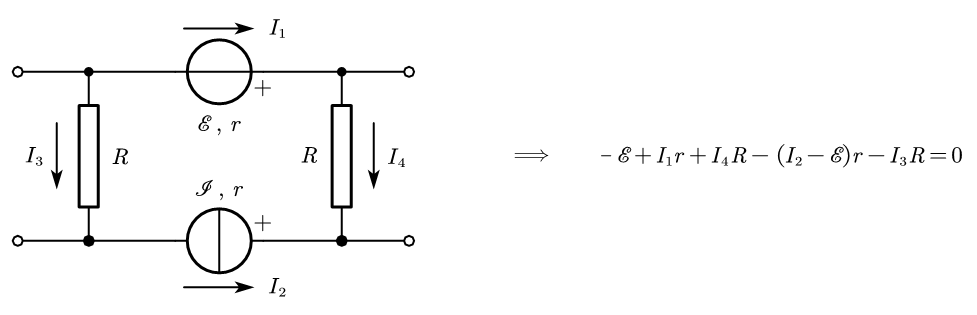
\includegraphics[width=0.8\textwidth]{image/7-3-12.png}
\caption{回路:\,数电压法}
\end{figure}

而节点电流也可以使用电压作为变量.\,另外还需要注意,\,利用数电压法我们可以得到KVL方程的一种非完整形式.\,由于我们对于节点总是喜欢定义其电势,\,那么如果节点$i,\,j$之间存在一条长的支路链,\,如下图所示,\,那么取$i\to j$方向为参考方向,\,电势降低就满足:

\begin{figure}[H]
\centering
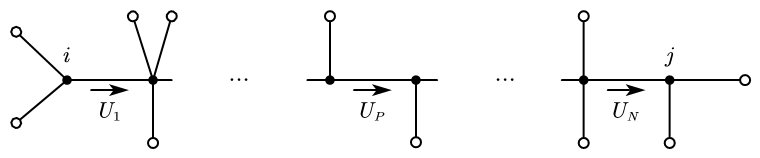
\includegraphics[width=0.6\textwidth]{image/7-3-13.png}
\caption{路径:\,数电压法}
\end{figure}

\vspace{-1cm}

\[\varphi_i-\varphi_j=\sum_P U_p\]

尤其是对于以后用得上的星型电阻网络问题,\,以三端为例,\,KCL或节点电流定律就可以在此时列为:
\begin{figure}[H]
\centering
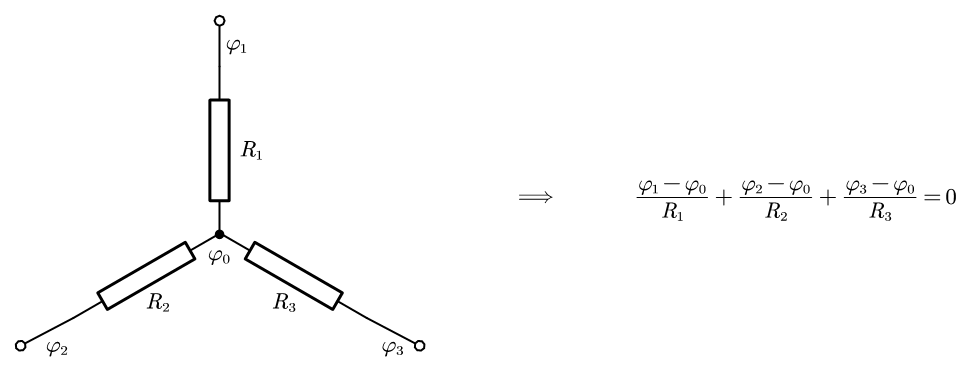
\includegraphics[width=0.65\textwidth]{image/7-3-14.png}
\caption{节点电压法使用KCL}
\end{figure}

一个典型的电路问题提法是如何?\,它又具有哪些元素与性质?\,解决方案又有哪些?\,我们下面从基础开始细细分析.


\section{电路分析基础}

\subsection{电路的整体结构与拓扑学结论}

电路分析中的以下三个重要概念的术语与立体几何学中的术语是可等值替换的:
\begin{itemize}
	\item 支路(branch)-边(edge)
	\item 节点(node)-顶点(vertex)
	\item 回路\footnote{注意,\,真正与面形成对应关系的应该是之后要引入的网孔的概念}(circuit)-面(face)
\end{itemize}

它们分别是什么含义?

最基础的概念莫过于支路.\,我们暂时采取最保守的做法,\,认为每一个元件都占据一个独立的支路,\,不同的支路之间可以是串联,\,并联,\,或者组合在一起的混联,\,或者什么也不是(典型的情况比如五条支路构成的桥式连接).

接下来定义节点的概念:\,节点把支路连接在一起.\,在定义这个概念时我们首次遇到了\emph{拓扑等价}(topological equivalence)的概念.\,众所周知,\,如果是用真实导线把真实的元件连接,\,那么连接方式不一定与电路图是完全对应的.\,事实上就电路图本身也具有一定的变化范围,\,比如对连接点的位移与导线的弯折具有等价性,\,如下图左.\,再比如说如果只允许电路图中出现三导线相交的情况时,\,把四个元件的一端相连就有如下图右的三种方式,\,当然,\,如果在中间红色导线上接上其他元件或是用理想电流表去测量其电流,\,那么这三个电路并不等价,\,但是如果只考虑下面要阐述的电路问题的标准提法的求解那么三个电路并无区别.
\begin{figure}[H]
\centering
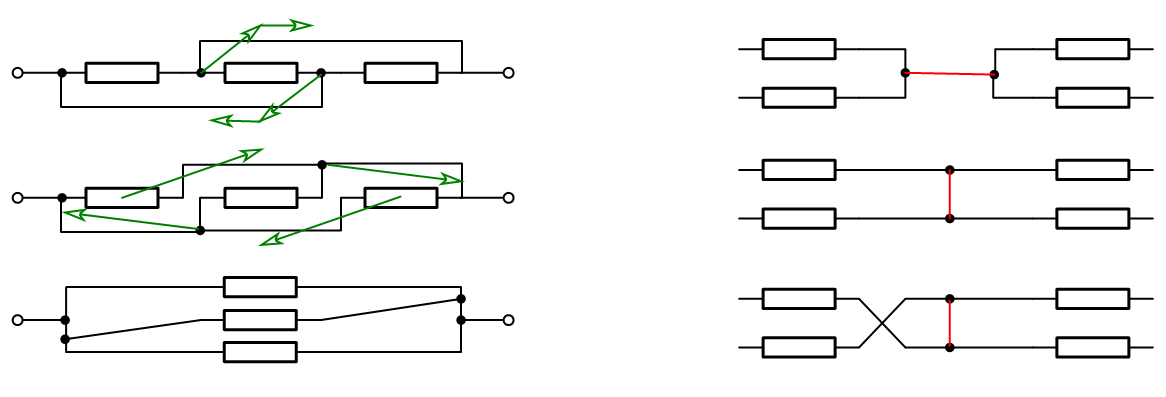
\includegraphics[width=0.65\textwidth]{image/7-3-15.png}
\caption{拓扑等价变形}
\end{figure}

既然电路可以被拓扑变形,\,那么节点的概念也就要被重新被考量了.\,事实上,\,节点相当于彼此等势的导线延伸体.\,导线无论如何连接与延伸,\,只要是彼此连通的点就被视作属于同一个节点.\,从这个视角上来看,\,上面的左图从一开始实际上就只有左右两个节点,\,右边的三个图中间全部都归为一个节点.

但是,\,出于几何上的直观,\,如果一个节点只被两个元件一端共用,\,那么这两个元件就称作\emph{串联}(series connection)的关系,\,两个元件的串联或多个元件的顺次串联的情况下,\,我们有理由把这一串元件全都视作在一条``强支路''上,\,原来的支路被\emph{合并},\,原来的中间的节点也就随着取消,\,剩下的节点至少应该是三条或三条以上的支路汇合的``强节点''.\,按照这种方式理解的强支路与强节点赋予电路以类似于多面体的拓扑结构.

\begin{wrapfigure}[10]{o}[-10pt]{6cm}
\centering
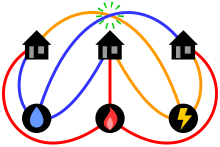
\includegraphics[width=6cm]{image/7-3-16.png}
\caption{三对三图$K_{3,3}$}
\end{wrapfigure}
要使得电路的结构完全类似于多面体,\,还缺少至关重要的一环:\,电路的回路就类似于多面体的面.\,电路的回路是由多段支路首尾相连构成的不相交的环.\,为了说明清楚回路分析中的重要一个因素:\,回路基.\,我们还需要引入\emph{可平面化图}(planar graph)的概念.\,我们知道,\,图是用来表示事物的连接关系的重要数学工具,\,在这个意义上就无所谓图所在空间的维数的说法.\,比如以右图表示的著名的\emph{三对三图}(three for three graph)中,\,有三户家庭分别都需要从水厂,\,气厂,\,电厂输送过来的资源,\,那么三户家庭与三个工厂看作节点,\,输送管道看作支路,\,这就构成了$K_{3,3}$图.\,当然任何维度空间中的网络,\,多面体的边与顶点自然也构成了一些图.\,但是原则上抽象为一个图以后就失去了任何抽象前的维度信息.\,这样就可以定义\emph{平面图}(plane graph):\,它是被画在一个平面上的,\,同时支路与支路没有相交的图.\,右边画的$K_{3,3}$图就不是一个平面图.\,事实上,\,它也不是一个可平面化图:\,可平面化图指的是虽然这个图可能以某种方式画在平面上支路会相交,\,但是总能找到使边不相交的办法.\,而著名的\emph{库拉托夫斯基定理}\footnote{直到1930年才被严格表述与证明.}(Kuratowski's theorem)指出:
\begin{quotation}
任何不可平面化的图,\,将串联支路合并后,\,必然包含一个五阶完全图\footnote{即五个点彼此连接}或三对三图为子图.
\end{quotation}

我们下面只研究平面图,\,但除了网孔概念以外,\,其余性质都是所有电路中的图共有的.

\vspace{0.5cm}
在平面图中\emph{网孔}(mesh)就是一个比较自然的概念了:\,平面图的每一个格子就是一个网孔.\,比如下图所示的三维立方体就产生了一个八节点十二支路的图.\,它是可以平面化的,\,按照右边的方式平面化以后,\,就会导致变成$5$个网孔的平面图.

\begin{figure}[H]
\centering
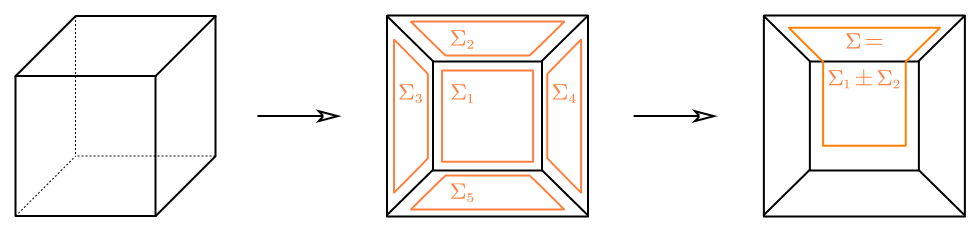
\includegraphics[width=0.8\textwidth]{image/7-3-17.png}
\caption{立方体的平面化与网孔合并为复杂回路}
\end{figure}

可以发现,\,网孔不过是特殊的一组回路.\,这些回路内部的平面区域已经不再有其他支路.\,如果网孔的个数为$F$,\,那么整个二维平面就被这些网孔回路分为$F+1$个区域,\,每个网孔内部是一个区域,\,而所有网孔外还有一个大的区域.

网孔作为一组特殊回路的特殊之处就在于,\,网孔是一组自然的\emph{回路基}(circuit basis).\,所谓回路独立就是指它们对应的回路电压方程独立,\,所谓回路基就是指所有可能回路的回路电压方程中选取的一组可以用来表示\footnote{通过方程的线性组合}所有其他方程的独立方程对应的独立回路.\,可以想见,\,回路的取法是远多于网孔的个数的,\,比如可以把上图两个相邻的网孔$\Sigma_1,\,\Sigma_2$合并为较大的回路$\Sigma$\footnote{从集合论的角度来讲,\,这种合并的本质是\emph{对称差}(symmetric difference),\,它被定义为:
\[A\triangle B=A\cup B-A\cap B\]

对于回路的合并这是很自然的:\,上式代表保留各自的边,\,去除公共边.\,但是对于回路合并对称差符号写为$\pm$符号是非常贴切的,\,因为容易理解对称差两次必然相互抵消:
\[(A\triangle B)\triangle B=A\]

从而从合并后的网孔去再次对称差合并前的网孔,\,又会回到合并的另一个网孔,\,像极了加减法:
\[\Sigma_1\pm \Sigma_2=\Sigma \quad \Leftrightarrow \quad \Sigma \pm \Sigma_2=\Sigma_1\]
}.\,所以回路基的取法并不是唯一的,\,原则上存在很多种独立回路的取法.

图论给出,\,对于任何一个电路图,\,都存在一个特征的数字:\,\emph{回路秩}\footnote{最早被\emph{基尔霍夫}({\it G. Kirchhoff})在1847年引入,\,当时称作\emph{圈数}(cyclomatic number).}(circuit rank),\,对于平面图它就是网孔的个数,\,对于非平面图可以用之后给出的办法计算.\,我们取一组最大数目的互相独立的回路做回路基时,\,其个数总是会等于这个回路秩.\,利用这个特性,\,即使是复杂的非平面电阻网络,\,只要我们总是避免选取的回路不独立,\,选够回路秩那么多回路时,\,就得到了一组回路基.

\vspace{1cm}

联系支路,\,节点,\,网孔(可换为回路基,\,下同)三者的最核心的定理,\,莫过于欧拉早在1758年就发现并证明的定理:\,如果一个三维空间中的没有洞的多面体(比如像甜甜圈那样,\,但是表面被磨为多个平面的多面体就是有洞的多面体)的顶点数为$V$,\,边数为$E$,\,而面数为$F$,\,那么必然有:
\[E=V+F-2\]

但是如果变成电路问题,\,由于多面体的面数与它所对应的被平面化的图的网孔数(或者图的回路秩,\,下同)总是差一.\,故对于电路问题,\,节点数$V$,\,支路数$E$和网孔数$F$三者满足的关系式应当为:
\[E=V+F-1\]

默认以上结果,\,就意味着我们终于具备了开始研究电路问题的数学基础.\,接下的第一步,\,就是严格的表述一个电路问题.


\begin{itemize}
\item 已知量:
	\begin{itemize}
	\item 首先,\,必须给定的是电路的拓扑,\,即已知电路由$V$个节点,\,$E$条支路构成,\,还应当能判断每一个节点$i$与每一条支路$P$之间是否有从属关系$i\in,\,\notin P$.
	\item 其次,\,每一条支路上的元件种类:\,电阻,\,恒压源或恒流源.\,与对应的参数$R,\,\mathscr{E},\,\mathscr{I},\,r$也应当事先给定.
	\end{itemize}
\item 待求量:
	\begin{itemize}
	\item 为每一条支路指定好方向以后,\,支路上的电流和电压都是待求的.\,由于电压电流通过支路元件特性相关联,\,一共$E$个未知数.
	\item 节点上的电势通常也是我们关心的,\,此时一般要约定好某节点接地视作零电势,\,其他节点的电势均是相对它的电势,\,都是待求量,\,一共$V-1$个未知数.
	\item 平面图形成了$F$个网孔.\,图论可以证明,\,因为满足KCL方程,\,合理的某种支路电流分布总存在唯一的某种\emph{网孔电流}(mesh current)的叠加与之等价.\,故也会产生对应的网孔电流待求量,\,一共$F$个未知数.
	\end{itemize}
\end{itemize}

网孔(回路)电流法是一种用来表示电路中的电流分布的快捷方法,\,其优点是自动会满足KCL方程.\,且未知数个数相对较少.\,其做法是:\,对于每个网孔$\Sigma$约定一个顺时针或逆时针的参考方向,\,并给定一个网孔电流$I_\Sigma$.\,那么对于每一条支路$P$,\,再为支路约定参考方向,\,则其上的电流等于:
\[I_P=\sum_{\Sigma\in P} \pm I_\Sigma\]

再一次地$\in$表示结合关系,\,$\Sigma\in P$念做``$\Sigma$以$P$为边''.\,需要注意,\,如果$\Sigma$就是取网孔,\,那么与任何一条支路发生结合关系的网孔最多只能有两个,\,即上式最多只有两项,\,而在图的边缘的支路则仅仅属于一个网孔.\,但是,\,如果取更广义地取回路基,\,则与同一条支路发生结合的回路个数可以是任意个.\,电流的符号需要根据回路电流的参考方向与后面对支路求和时的方向是否相同来决定,\,同向取正,\,反向取负.\,下图对同一个平面电路图,\,用网孔电流法和回路电流法分别表示两条代表性支路上的电流:

\begin{figure}[H]
\centering
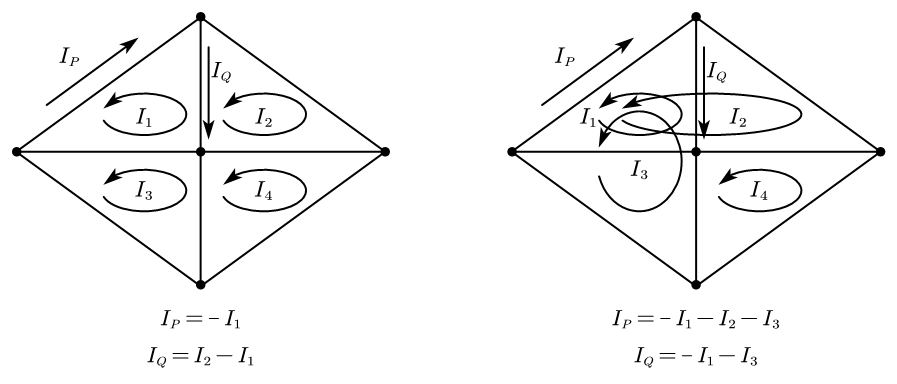
\includegraphics[width=0.65\textwidth]{image/7-3-18.png}
\caption{网孔(回路)电流法}
\end{figure}

最后,\,通过已知量求未知量的方法,\,应当是各类KCL和KVL方程.\,它们应当如何列,\,列多少个?\,这就形成了电路问题的求解套路:

\subsection{电路问题的求解套路}

电路问题的求解有三种套路:\,支路电流法,\,节点电势法和网孔(回路)电流法.\,无论采用哪一种方法,\,无非是对之前梳理的三类待求量中,\,选取一类集中加以解决:\,解决的方案无非是设它们为未知数,\,并找到与未知数的个数恰好相等的,\,包含且仅包含这些未知数的KCL或KVL方程,\,这必然得到线性方程组.\,解出它们并根据它们得到另外两类待求量.\,下面逐一论述之.

\vspace{0.2cm}
\textbf{1.\,支路电流法}
\vspace{0.2cm}

如果为每一条支路约定好参考方向,\,并设其上电流为$I_P$,\,则一共有$E$个未知数.

我们需要列出几乎全套的KCL,\,对每一个节点$i$,\,这个方程写作:
\[\sum_{P\in i} \pm I_P=0\]

正负号约定是:\,如果支路电流参考方向为指向该节点,\,则取正,\,若背离该节点,\,则取负.\,但是所有的KCL放在一起并不独立,\,这是因为所有的KCL方程求和后,\,每一条支路的$I_P$恰好在两端点处的KCL中出现两次,\,一正一负,\,故最后得到零等于零.\,从而需要去掉一个任意节点$j$,\,即可以列出$V-1$个方程:
\[\forall i\neq j \quad ,\quad \sum_{P\in i} \pm I_P=0\]

对于每一个网孔还要列一个KVL方程,\,为了方便与统一起见,\,我们把所有带内阻的恒流源都变成等效的带内阻恒压源,\,而电阻元件也视作$\mathscr{E}=0$的特殊情况,\,下同.\,这样KVL方程中的电压就可以用电流表示,\,一共是$F$个方程:
\[\forall \Sigma \quad ,\quad \sum_{P\in \Sigma } \pm U_P=0\]
\[U_P=-\mathscr{E}_P+I_P R_P \]

正负号约定是,\,如果约定回路的环绕方向与支路参考方向一致则取正,\,相反则取负.

整理,\,对以上KVL方程把未知数置于左侧,\,常数(非齐次项)置于右侧,\,得到:
\[\forall i\neq j \quad ,\quad \sum_{P\in i} \pm I_P=0\]
\[\forall \Sigma \quad ,\quad \sum_{P\in \Sigma } \pm R_P I_P=\sum_{P\in \Sigma } \pm \mathscr{E}_P\]

一共是$V-1+F$个方程,\,恰好等于未知数的个数$E$,\,因为:
\[E=V+F-1\]

\vspace{0.2cm}
\textbf{2.\,节点电势法}
\vspace{0.2cm}

如果为某个节点$j$接地,\,即约定其电势为$\varphi_j=0$,\,对其他节点$i\neq j$设电势$\varphi_i$,\,则一共有$V-1$个未知数.\,此时KVL方程已经给不出有意义的方程,\,只能列KCL方程.\,任何一条支路$P$,\,如果两端点为$i,\,k$,\,那么如果约定$i$到$k$方向为其参考方向,\,有:
\[U_P=\varphi_i-\varphi_k =- \mathscr{E}_P+ I_PR_P \quad \Rightarrow \quad I_P=\frac{\varphi_i}{R_P}-\frac{\varphi_k}{R_P}+\frac{\mathscr{E}_P}{R_P}\]

那么根据KCL方程,\,所有流入$k$节点的电流应当和为零:
\[\left(\sum_{P\in k}\frac{1}{R_P}\right)\varphi_k-\sum_{i\in P\in k}\left(\frac{1}{R_P}\varphi_i\right)=\sum_{P\in k}\frac{\mathscr{E}_P}{R_P}\]

其中$i\in P\in k$念做$i,\,j通过P相连$.\,同样的,\,这$V$个方程并不独立,\,应当再去掉一个$k$的方程,\,由于$\varphi_j=0$不必解,\,不妨就去掉这一个,\,并使左侧不出现$\varphi_j$:
\[\forall k\neq j\quad ,\quad \left(\sum_{P\in k}\frac{1}{R_P}\right)\varphi_k-\sum_{\substack{i\in P\in k\\ i\neq j}}\left(\frac{1}{R_P}\varphi_i\right)=\sum_{P\in k}\frac{\mathscr{E}_P}{R_P}\]

这样方程数也是$V-1$个,\,等于未知数个数$V_1$.

\vspace{0.2cm}
\textbf{3.\,网孔电流法}
\vspace{0.2cm}

如果对每个网孔,\,约定参考方向后设每个网孔电流为$I_\Sigma$,\,则一共有$F$个未知数.\,此时KCL方程已经给不出有意义的方程,\,只能列KVL方程.\,任何一条支路$P\in \Sigma$,\,如果按照所在网孔$\Sigma$的参考方向,\,有:
\[U_P=-\mathscr{E}_P+I_PR_P=-\mathscr{E}_P+R_P\sum_{\Pi \in P}\pm I_\Pi\]

求和中恰好有一项就是原来的$I_\Sigma$,\,它取正号,\,而其他的回路$\Pi$应当根据与回路$\Sigma$在公共边$P$上的方向是否一致来决定正负号,\,同向为正,\,反向为负.\,将上式求和得到KVL:
\[\forall \Sigma\quad ,\quad \left(\sum_{P\in\Sigma}R_P\right)I_\Sigma+\sum_{P\in\Sigma}\left(R_P\sum_{\Pi \in P\in \Sigma}\pm I_\Pi\right)=\sum_{P\in\Sigma}\mathscr{E}_P \]

其中$\Pi \in P\in \Sigma$念做``$\Pi$和$\Sigma$共用边$P$''.\,这样方程数也是$F$个,\,等于未知数个数$F$.

\vspace{0.5cm}

一方面,\,三种方法的未知数与方程个数分别是$E,\,V-1,\,F$,\,而$E=V-1+F$,\,所以显然后两种方法的未知数和方程数都是比第一种少的,\,在实际应用过程中更加省事,\,原则上我们应当尽可能地使用后两种方法来解决实际问题.\,但是另一方面,\,第一种方法得到的方程形式上更简洁而易于分析,\,所以理论推导的时候也青睐基础的支路电流法.

\section{电路分析方法}
%往往,\,我们不希望把整个电路的解全都找到,\,而只关心个别元件上的电压,\,电流.\,这样之前的完整求解的套路就瞬间失去了意义.\,反倒是各种等效的方法大放异彩.\,这一节我们主要的线索就是来探讨各式各样等效原理的来龙去脉,\,它们起到了化简电路的实际作用.

%\subsection{二端电路等效}

%\begin{figure}[H]
%\centering
%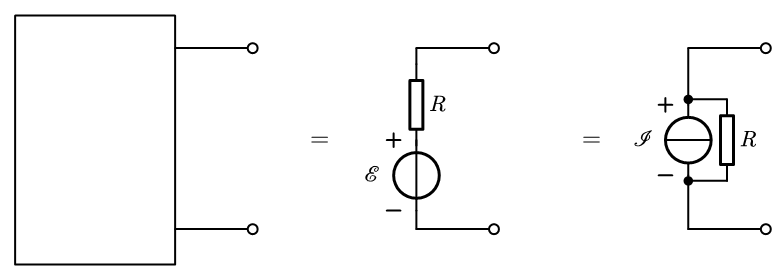
\includegraphics[width=0.65\textwidth]{image/7-3-19.png}
%\caption{等效原理}
%\end{figure}

\begin{itemize}
\item 叠加原理:\,用上一节介绍的任何一种方法求解方程组时,\,右边的非齐次项都可以进行拆分与叠加.\,直接推论是,\,如果电路只含电压源,\,那么保留各个单个电压源,\,其他电压源置零,\,解出的各支路电流的和即每个电压源都存在时的电流.

\item 任何二端不含源电阻网络都可以等效为一个线性电阻.

\item 戴维南-诺尔顿原理:\,任何二端含源网络如果把各电压源电流源置零之后形成的不含源电阻网络的等效电阻网络电阻为$r$,\,其开路电压$U$,\,其短路电流$I$.\,那么这个电路等效于一个电压源或电流源,\,内阻即$r$,\,电压或电流即$U,\,I$.

\item 特勒根原理:\,单一电路中若各个支路选取相关方向,\,则:
\[\sum_P U_PI_P=0\]

如果两个电路的图一样,\,即具有相同的节点,\,支路,\,网孔结构,\,但是元件可以不一样.\,那么选取各个支路为相关方向,\,也有:
\[\sum_P U_{1P}I_{2P}=0=\sum_P U_{2P}I_{1P}\]
\end{itemize}


%\section{半导体}
